\documentclass[11pt,letterpaper]{article}

% ============================================================================
% PACKAGES
% ============================================================================
\usepackage[utf8]{inputenc}
\usepackage[T1]{fontenc}
\usepackage{geometry}
\usepackage{graphicx}
\usepackage{xcolor}
\usepackage{tikz}
\usepackage{tcolorbox}
\usepackage{booktabs}
\usepackage{array}
\usepackage{longtable}
\usepackage{amsmath}
\usepackage{amssymb}
\usepackage{enumitem}
\usepackage{fancyhdr}
\usepackage{titlesec}
\usepackage{hyperref}
\usepackage{multirow}
\usepackage{tabularx}
\usepackage{float}
\usepackage{caption}
\usepackage{subcaption}
\usepackage{setspace}
\usepackage{parskip}
\usepackage{pdflscape}
\usepackage{afterpage}
\usepackage{colortbl}

% ============================================================================
% PAGE LAYOUT
% ============================================================================
\geometry{
    left=1in,
    right=1in,
    top=1in,
    bottom=1in,
    headheight=24pt
}

% ============================================================================
% COLORS
% ============================================================================
\definecolor{primaryblue}{RGB}{0, 82, 147}
\definecolor{secondaryblue}{RGB}{52, 152, 219}
\definecolor{accentgreen}{RGB}{39, 174, 96}
\definecolor{warningorange}{RGB}{230, 126, 34}
\definecolor{alertred}{RGB}{192, 57, 43}
\definecolor{lightgray}{RGB}{245, 245, 245}
\definecolor{darkgray}{RGB}{64, 64, 64}
\definecolor{purple}{RGB}{142, 68, 173}
\definecolor{teal}{RGB}{22, 160, 133}
\definecolor{phase1}{RGB}{46, 134, 193}
\definecolor{phase2}{RGB}{40, 180, 99}
\definecolor{phase3}{RGB}{243, 156, 18}
\definecolor{phase4}{RGB}{155, 89, 182}
\definecolor{phase5}{RGB}{231, 76, 60}

% ============================================================================
% TIKZ LIBRARIES
% ============================================================================
\usetikzlibrary{shapes.geometric, arrows.meta, positioning, calc, fit, backgrounds, matrix, decorations.pathreplacing, shapes.multipart, patterns, shadows}

% ============================================================================
% TCOLORBOX STYLES
% ============================================================================
\tcbuselibrary{skins, breakable}

\newtcolorbox{keyconceptbox}[1][]{
    colback=primaryblue!5,
    colframe=primaryblue,
    fonttitle=\bfseries,
    title=#1,
    breakable,
    enhanced,
    boxrule=1pt,
    left=8pt,
    right=8pt,
    top=6pt,
    bottom=6pt
}

\newtcolorbox{examplebox}[1][]{
    colback=accentgreen!5,
    colframe=accentgreen,
    fonttitle=\bfseries,
    title=#1,
    breakable,
    enhanced,
    boxrule=1pt,
    left=8pt,
    right=8pt,
    top=6pt,
    bottom=6pt
}

\newtcolorbox{notebox}[1][]{
    colback=warningorange!5,
    colframe=warningorange,
    fonttitle=\bfseries,
    title=#1,
    breakable,
    enhanced,
    boxrule=1pt,
    left=8pt,
    right=8pt,
    top=6pt,
    bottom=6pt
}

\newtcolorbox{alertbox}[1][]{
    colback=alertred!5,
    colframe=alertred,
    fonttitle=\bfseries,
    title=#1,
    breakable,
    enhanced,
    boxrule=1pt,
    left=8pt,
    right=8pt,
    top=6pt,
    bottom=6pt
}

\newtcolorbox{summarybox}{
    colback=lightgray,
    colframe=darkgray,
    breakable,
    enhanced,
    boxrule=1pt,
    left=8pt,
    right=8pt,
    top=6pt,
    bottom=6pt
}

\newtcolorbox{policybox}[1][]{
    colback=purple!5,
    colframe=purple,
    fonttitle=\bfseries,
    title=#1,
    breakable,
    enhanced,
    boxrule=1pt,
    left=8pt,
    right=8pt,
    top=6pt,
    bottom=6pt
}

\newtcolorbox{milestonebox}[1][]{
    colback=teal!5,
    colframe=teal,
    fonttitle=\bfseries,
    title=#1,
    breakable,
    enhanced,
    boxrule=1pt,
    left=8pt,
    right=8pt,
    top=6pt,
    bottom=6pt
}

\newtcolorbox{phasebox}[2][]{
    colback=#2!8,
    colframe=#2,
    fonttitle=\bfseries\large,
    title=#1,
    breakable,
    enhanced,
    boxrule=1.5pt,
    left=10pt,
    right=10pt,
    top=8pt,
    bottom=8pt,
    drop shadow
}

% ============================================================================
% HEADER AND FOOTER
% ============================================================================
\pagestyle{fancy}
\fancyhf{}
\fancyhead[L]{\textcolor{primaryblue}{\small Application Security Program Roadmap}}
\fancyhead[R]{\textcolor{primaryblue}{\small Implementation Guide}}
\fancyfoot[C]{\thepage}
\renewcommand{\headrulewidth}{0.5pt}
\renewcommand{\headrule}{\hbox to\headwidth{\color{primaryblue}\leaders\hrule height \headrulewidth\hfill}}

% ============================================================================
% SECTION FORMATTING
% ============================================================================
\titleformat{\section}
    {\Large\bfseries\color{primaryblue}}
    {\thesection}{1em}{}
\titleformat{\subsection}
    {\large\bfseries\color{secondaryblue}}
    {\thesubsection}{1em}{}
\titleformat{\subsubsection}
    {\normalsize\bfseries\color{darkgray}}
    {\thesubsubsection}{1em}{}

% ============================================================================
% HYPERREF SETUP
% ============================================================================
\hypersetup{
    colorlinks=true,
    linkcolor=primaryblue,
    urlcolor=secondaryblue,
    citecolor=accentgreen,
    pdftitle={Application Security Program Roadmap},
    pdfauthor={Security Organization},
    pdfsubject={Comprehensive Implementation Roadmap for Enterprise Application Security}
}

% ============================================================================
% CUSTOM COMMANDS
% ============================================================================
\newcommand{\risk}[1]{\textcolor{alertred}{\textbf{#1}}}
\newcommand{\control}[1]{\textcolor{accentgreen}{\textbf{#1}}}
\newcommand{\process}[1]{\textcolor{primaryblue}{\textbf{#1}}}
\newcommand{\milestone}[1]{\textcolor{teal}{\textbf{#1}}}
\newcommand{\quarter}[1]{\textbf{Q#1}}
\newcommand{\pmark}{\textcolor{accentgreen}{\checkmark}}
\newcommand{\ongoing}{\textcolor{secondaryblue}{$\circlearrowright$}}

% ============================================================================
% DOCUMENT BEGINS
% ============================================================================
\begin{document}

% ============================================================================
% TITLE PAGE
% ============================================================================
\begin{titlepage}
    \centering
    \vspace*{0.5cm}
    
    {\Huge\bfseries\textcolor{primaryblue}{Application Security\\Program Roadmap}\par}
    
    \vspace{0.5cm}
    
    {\LARGE\textcolor{secondaryblue}{Strategic Implementation Guide for\\Enterprise Security Excellence}\par}
    
    \vspace{1.5cm}
    
    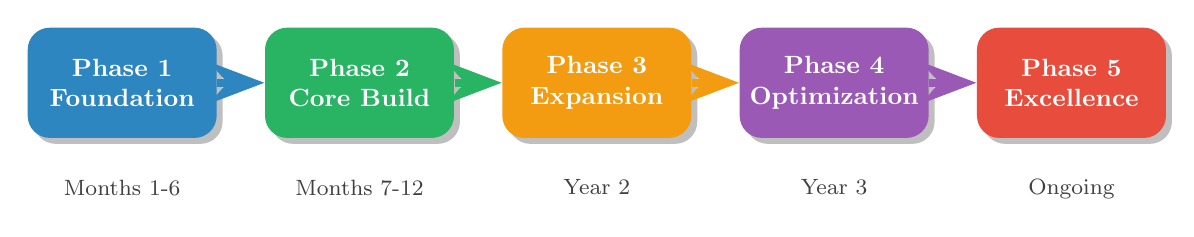
\begin{tikzpicture}[
        node distance=0.6cm,
        phasearrow/.style={-{Stealth[scale=1.2]}, line width=3pt},
        phasenode/.style={rectangle, rounded corners=8pt, minimum width=2.4cm, minimum height=1.4cm, align=center, font=\small\bfseries, text=white, drop shadow}
    ]
        % Phase nodes
        \node[phasenode, fill=phase1] (p1) {Phase 1\\Foundation};
        \node[phasenode, fill=phase2, right=of p1] (p2) {Phase 2\\Core Build};
        \node[phasenode, fill=phase3, right=of p2] (p3) {Phase 3\\Expansion};
        \node[phasenode, fill=phase4, right=of p3] (p4) {Phase 4\\Optimization};
        \node[phasenode, fill=phase5, right=of p4] (p5) {Phase 5\\Excellence};
        
        % Arrows
        \draw[phasearrow, phase1] (p1) -- (p2);
        \draw[phasearrow, phase2] (p2) -- (p3);
        \draw[phasearrow, phase3] (p3) -- (p4);
        \draw[phasearrow, phase4] (p4) -- (p5);
        
        % Timeline
        \node[below=0.4cm of p1, font=\footnotesize\color{darkgray}] {Months 1-6};
        \node[below=0.4cm of p2, font=\footnotesize\color{darkgray}] {Months 7-12};
        \node[below=0.4cm of p3, font=\footnotesize\color{darkgray}] {Year 2};
        \node[below=0.4cm of p4, font=\footnotesize\color{darkgray}] {Year 3};
        \node[below=0.4cm of p5, font=\footnotesize\color{darkgray}] {Ongoing};
    \end{tikzpicture}
    
    \vspace{1.5cm}
    
    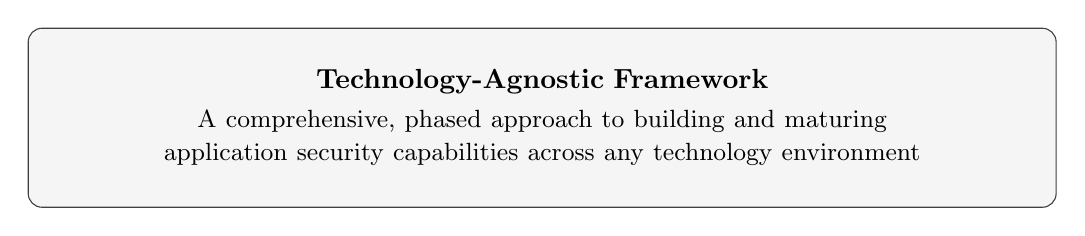
\begin{tikzpicture}
        \node[draw=darkgray, fill=lightgray, rounded corners=5pt, 
              text width=12cm, align=center, inner sep=15pt] {
            \textbf{Technology-Agnostic Framework}\\[0.3em]
            {\small A comprehensive, phased approach to building and maturing\\application security capabilities across any technology environment}
        };
    \end{tikzpicture}
    
    \vspace{1.5cm}
    
    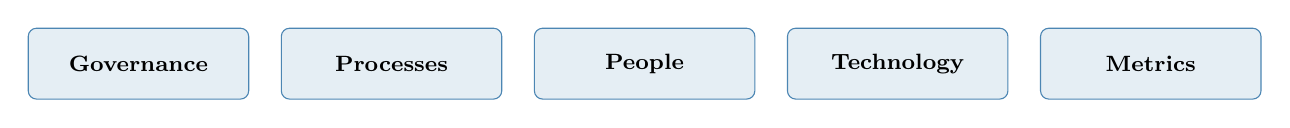
\begin{tikzpicture}[
        node distance=0.4cm,
        pillar/.style={rectangle, draw=primaryblue!70, fill=primaryblue!10, rounded corners=3pt, minimum width=2.8cm, minimum height=0.9cm, align=center, font=\footnotesize\bfseries}
    ]
        \node[pillar] (gov) {Governance};
        \node[pillar, right=of gov] (proc) {Processes};
        \node[pillar, right=of proc] (people) {People};
        \node[pillar, right=of people] (tech) {Technology};
        \node[pillar, right=of tech] (metrics) {Metrics};
    \end{tikzpicture}
    
    \vfill
    
    {\large\textcolor{darkgray}{Version 2.0}\par}
    \vspace{0.3cm}
    {\large\textcolor{darkgray}{\today}\par}
    
\end{titlepage}

% ============================================================================
% TABLE OF CONTENTS
% ============================================================================
\newpage
\tableofcontents
\newpage

% ============================================================================
% SECTION 1: EXECUTIVE SUMMARY
% ============================================================================
\section{Executive Summary}

This Application Security Program Roadmap provides a comprehensive, phased approach to implementing and maturing enterprise application security capabilities. The roadmap is technology-agnostic, designed to apply across any platform, programming language, architecture, or deployment model, enabling organizations to build security capabilities that adapt to their unique technology environment.

\begin{keyconceptbox}[Roadmap Purpose]
This roadmap transforms the Application Security Program framework into actionable implementation guidance, providing specific activities, milestones, resource requirements, and success criteria for each phase of program development. It enables organizations to systematically build security capabilities while demonstrating measurable progress to stakeholders.
\end{keyconceptbox}

\subsection{Strategic Objectives}

The roadmap pursues the following strategic objectives across its implementation phases:

\begin{enumerate}[leftmargin=2em, itemsep=0.4em]
    \item \textbf{Establish Governance Foundation:} Create the organizational structures, policies, and accountability mechanisms necessary to sustain long-term security improvement.
    
    \item \textbf{Build Core Capabilities:} Implement essential security testing, vulnerability management, and secure development practices that address the most critical risks.
    
    \item \textbf{Achieve Comprehensive Coverage:} Extend security activities across the entire application portfolio with appropriate depth based on risk classification.
    
    \item \textbf{Optimize for Efficiency:} Mature processes and automation to reduce friction, improve developer experience, and maximize security return on investment.
    
    \item \textbf{Enable Continuous Evolution:} Establish sustainable practices for ongoing improvement, adaptation to emerging threats, and maintenance of security excellence.
\end{enumerate}

\subsection{Roadmap Structure}

The implementation roadmap spans approximately three years of active development followed by ongoing continuous improvement. The phased approach allows organizations to demonstrate early value while building toward comprehensive security coverage.

\begin{figure}[H]
\centering
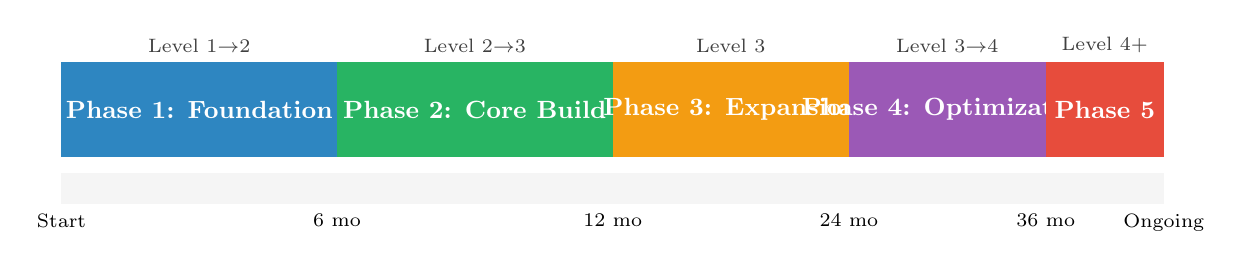
\begin{tikzpicture}[
    node distance=0.15cm,
    timeline/.style={rectangle, minimum width=14cm, minimum height=0.6cm, align=center, font=\small},
    phase/.style={rectangle, rounded corners=3pt, minimum height=1.2cm, align=center, font=\small\bfseries, text=white}
]
    % Timeline bar
    \fill[lightgray] (0,0) rectangle (14,0.4);
    
    % Phase bars
    \fill[phase1] (0,0.6) rectangle (3.5,1.8);
    \node[text=white, font=\small\bfseries] at (1.75,1.2) {Phase 1: Foundation};
    
    \fill[phase2] (3.5,0.6) rectangle (7,1.8);
    \node[text=white, font=\small\bfseries] at (5.25,1.2) {Phase 2: Core Build};
    
    \fill[phase3] (7,0.6) rectangle (10,1.8);
    \node[text=white, font=\small\bfseries] at (8.5,1.2) {Phase 3: Expansion};
    
    \fill[phase4] (10,0.6) rectangle (12.5,1.8);
    \node[text=white, font=\small\bfseries] at (11.25,1.2) {Phase 4: Optimization};
    
    \fill[phase5] (12.5,0.6) rectangle (14,1.8);
    \node[text=white, font=\small\bfseries] at (13.25,1.2) {Phase 5};
    
    % Time labels
    \node[below, font=\scriptsize] at (0,0) {Start};
    \node[below, font=\scriptsize] at (3.5,0) {6 mo};
    \node[below, font=\scriptsize] at (7,0) {12 mo};
    \node[below, font=\scriptsize] at (10,0) {24 mo};
    \node[below, font=\scriptsize] at (12.5,0) {36 mo};
    \node[below, font=\scriptsize] at (14,0) {Ongoing};
    
    % Maturity labels
    \node[above, font=\scriptsize\color{darkgray}] at (1.75,1.8) {Level 1$\rightarrow$2};
    \node[above, font=\scriptsize\color{darkgray}] at (5.25,1.8) {Level 2$\rightarrow$3};
    \node[above, font=\scriptsize\color{darkgray}] at (8.5,1.8) {Level 3};
    \node[above, font=\scriptsize\color{darkgray}] at (11.25,1.8) {Level 3$\rightarrow$4};
    \node[above, font=\scriptsize\color{darkgray}] at (13.25,1.8) {Level 4+};
\end{tikzpicture}
\caption{Roadmap Timeline and Maturity Progression}
\label{fig:roadmap-timeline}
\end{figure}

\clearpage
\subsection{Key Success Factors}

\begin{summarybox}
\textbf{Critical Success Factors for Roadmap Execution:}

\textbf{1. Executive Sponsorship:} Active, visible support from C-level leadership with authority to allocate resources and enforce security requirements across the organization.

\textbf{2. Adequate Resourcing:} Commitment to staffing, tooling, and budget allocations specified in the resource requirements for each phase.

\textbf{3. Cultural Alignment:} Organization-wide acceptance that security is a shared responsibility integrated into development workflows rather than a separate gate.

\textbf{4. Phased Approach:} Disciplined execution of each phase with clear completion criteria before advancing to subsequent phases.

\textbf{5. Measurable Progress:} Regular tracking and reporting of metrics that demonstrate value and identify improvement opportunities.

\textbf{6. Adaptive Execution:} Willingness to adjust timelines and priorities based on organizational context, emerging threats, and lessons learned.

\textbf{7. Stakeholder Engagement:} Ongoing communication with development teams, business units, and leadership to maintain alignment and address concerns.
\end{summarybox}

\subsection{Document Organization}

This roadmap document is organized into the following major sections:

\begin{itemize}[leftmargin=2em]
    \item \textbf{Section 2: Pre-Implementation Assessment} --- Readiness evaluation and baseline establishment
    \item \textbf{Section 3: Phase 1 - Foundation} --- Governance, initial capabilities, and quick wins
    \item \textbf{Section 4: Phase 2 - Core Build} --- Essential security testing and vulnerability management
    \item \textbf{Section 5: Phase 3 - Expansion} --- Portfolio-wide coverage and advanced capabilities
    \item \textbf{Section 6: Phase 4 - Optimization} --- Process maturation and efficiency improvements
    \item \textbf{Section 7: Phase 5 - Excellence} --- Continuous evolution and industry leadership
    \item \textbf{Section 8: Resource Requirements} --- Staffing, budget, and tooling needs
    \item \textbf{Section 9: Risk Management} --- Implementation risks and mitigation strategies
    \item \textbf{Section 10: Governance and Oversight} --- Program management and reporting
    \item \textbf{Appendices} --- Templates, checklists, and reference materials
\end{itemize}

% ============================================================================
% SECTION 2: PRE-IMPLEMENTATION ASSESSMENT
% ============================================================================
\clearpage
\section{Pre-Implementation Assessment}

Before beginning roadmap execution, organizations must assess their current security posture, organizational readiness, and implementation context. This assessment establishes the baseline from which progress will be measured and identifies factors that may require roadmap customization.

\subsection{Current State Assessment}

\subsubsection{Application Portfolio Analysis}

Understanding the application landscape is fundamental to effective roadmap planning. The portfolio analysis should capture:

\begin{table}[H]
\centering
\renewcommand{\arraystretch}{1.3}
\begin{tabularx}{\textwidth}{>{\bfseries}p{3.5cm} X}
\toprule
\textbf{Assessment Area} & \textbf{Information to Gather} \\
\midrule
Inventory Completeness & Total number of applications; completeness of current inventory; applications not yet catalogued; shadow IT assessment \\
Technology Distribution & Programming languages in use; frameworks and platforms; deployment models (on-premises, cloud, hybrid); containerization and orchestration usage \\
Data Classification & Applications processing sensitive data categories; regulatory scope (PCI, HIPAA, GDPR, etc.); data flow mapping completeness \\
Business Criticality & Revenue-generating applications; customer-facing applications; internal enterprise applications; development and test environments \\
Development Practices & SDLC methodologies in use; CI/CD adoption level; code repository structure; deployment frequency \\
Third-Party Components & Open-source usage patterns; commercial component dependencies; API integrations; SaaS dependencies \\
\bottomrule
\end{tabularx}
\caption{Application Portfolio Assessment Dimensions}
\label{tab:portfolio-assessment}
\end{table}

\clearpage
\subsubsection{Security Capability Baseline}

Assess existing security capabilities across the following dimensions:

\begin{table}[H]
\centering
\renewcommand{\arraystretch}{1.3}
\begin{tabularx}{\textwidth}{>{\bfseries}p{3cm} p{4cm} X}
\toprule
\textbf{Capability Area} & \textbf{Current State Questions} & \textbf{Evidence to Collect} \\
\midrule
Governance & Existing policies? Defined roles? Executive support? & Policy documents; org charts; meeting minutes \\
Security Testing & Tools deployed? Coverage percentage? Integration level? & Tool inventory; scan reports; pipeline configs \\
Vulnerability Mgmt & Tracking system? SLAs defined? Remediation rates? & Tracking data; historical trends; open vuln counts \\
Secure Development & Training provided? Secure coding standards? Code review practices? & Training records; standards docs; review procedures \\
Incident Response & Defined procedures? Past incidents? Response capabilities? & IR plans; incident logs; post-mortems \\
Metrics \& Reporting & Metrics collected? Dashboards available? Reporting cadence? & Current reports; data sources; stakeholder feedback \\
\bottomrule
\end{tabularx}
\caption{Security Capability Baseline Assessment}
\label{tab:capability-baseline}
\end{table}

\clearpage
\subsubsection{Maturity Assessment}

Conduct a formal maturity assessment to establish baseline capability levels. The assessment should evaluate each program domain against a standardized maturity scale:

\begin{table}[H]
\centering
\renewcommand{\arraystretch}{1.4}
\begin{tabularx}{\textwidth}{>{\bfseries\centering\arraybackslash}p{1.5cm} p{2.5cm} X}
\toprule
\textbf{Level} & \textbf{Designation} & \textbf{Characteristics} \\
\midrule
0 & Non-Existent & No formal security activities; ad-hoc responses to incidents \\
1 & Initial & Some awareness; inconsistent practices; reactive approach; individual efforts \\
2 & Developing & Documented processes; partial implementation; limited tooling; inconsistent execution \\
3 & Defined & Standardized processes; organization-wide policies; systematic execution; established metrics \\
4 & Managed & Quantitative management; proactive optimization; integrated tooling; predictable outcomes \\
5 & Optimizing & Continuous improvement; innovation focus; industry leadership; adaptive capabilities \\
\bottomrule
\end{tabularx}
\caption{Maturity Level Definitions}
\label{tab:maturity-levels}
\end{table}

\begin{examplebox}[Maturity Assessment Template]
Rate each capability area from 0-5 based on the maturity level definitions:

\begin{tabular}{p{5cm} c c c}
\textbf{Capability Area} & \textbf{Current} & \textbf{Year 1 Target} & \textbf{Year 3 Target} \\
\midrule
Security Governance & \_\_\_ & \_\_\_ & \_\_\_ \\
Policy \& Standards & \_\_\_ & \_\_\_ & \_\_\_ \\
Risk Management & \_\_\_ & \_\_\_ & \_\_\_ \\
Secure Architecture & \_\_\_ & \_\_\_ & \_\_\_ \\
Secure Development & \_\_\_ & \_\_\_ & \_\_\_ \\
Security Testing (SAST) & \_\_\_ & \_\_\_ & \_\_\_ \\
Security Testing (DAST) & \_\_\_ & \_\_\_ & \_\_\_ \\
Security Testing (SCA) & \_\_\_ & \_\_\_ & \_\_\_ \\
Vulnerability Management & \_\_\_ & \_\_\_ & \_\_\_ \\
Security Training & \_\_\_ & \_\_\_ & \_\_\_ \\
Metrics \& Reporting & \_\_\_ & \_\_\_ & \_\_\_ \\
Incident Response & \_\_\_ & \_\_\_ & \_\_\_ \\
\end{tabular}
\end{examplebox}

\clearpage
\subsection{Organizational Readiness}

\subsubsection{Stakeholder Analysis}

Identify and assess key stakeholders who will influence or be affected by the program:

\begin{table}[H]
\centering
\renewcommand{\arraystretch}{1.3}
\begin{tabularx}{\textwidth}{>{\bfseries}p{3cm} p{3cm} X}
\toprule
\textbf{Stakeholder Group} & \textbf{Influence Level} & \textbf{Key Concerns to Address} \\
\midrule
Executive Leadership & High & ROI demonstration; risk reduction; regulatory compliance \\
Development Teams & High & Workflow integration; false positive rates; remediation burden \\
IT Operations & Medium-High & Deployment impact; tool integration; operational overhead \\
Product Management & Medium & Release timelines; feature priorities; customer impact \\
Legal/Compliance & Medium & Regulatory requirements; liability; policy enforcement \\
Business Units & Varies & Application availability; project timelines; resource competition \\
Internal Audit & Medium & Control effectiveness; evidence availability; finding remediation \\
\bottomrule
\end{tabularx}
\caption{Stakeholder Analysis Matrix}
\label{tab:stakeholder-analysis}
\end{table}

\subsubsection{Organizational Enablers and Barriers}

Assess factors that will enable or impede successful implementation:

\begin{table}[H]
\centering
\renewcommand{\arraystretch}{1.3}
\begin{tabularx}{\textwidth}{>{\bfseries}p{3cm} X X}
\toprule
\textbf{Factor} & \textbf{Enablers} & \textbf{Barriers} \\
\midrule
Leadership & Active sponsorship; security prioritization; resource commitment & Competing priorities; security seen as cost center; limited authority \\
Culture & Quality focus; continuous improvement mindset; collaboration & Blame culture; siloed teams; resistance to change \\
Resources & Available budget; skilled personnel; tool access & Budget constraints; talent shortage; legacy technical debt \\
Processes & Existing SDLC; CI/CD pipelines; change management & Manual processes; inconsistent practices; lack of standards \\
Technology & Modern architecture; centralized repositories; API-driven tools & Legacy systems; fragmented tooling; integration challenges \\
\bottomrule
\end{tabularx}
\caption{Organizational Enabler and Barrier Assessment}
\label{tab:enablers-barriers}
\end{table}

\subsubsection{Risk Appetite Alignment}

Document the organization's risk appetite for application security to ensure roadmap priorities align with business expectations:

\begin{alertbox}[Risk Appetite Considerations]
\begin{itemize}[leftmargin=1.5em, itemsep=0.2em]
    \item What level of residual risk is acceptable for different application tiers?
    \item How does the organization balance security investment against delivery speed?
    \item What security incidents would be considered unacceptable?
    \item What regulatory or contractual requirements are non-negotiable?
    \item How much development velocity impact is acceptable for security controls?
\end{itemize}
\end{alertbox}

\clearpage
\subsection{Roadmap Customization Factors}

Based on assessment findings, identify factors that may require roadmap customization:

\begin{table}[H]
\centering
\renewcommand{\arraystretch}{1.3}
\begin{tabularx}{\textwidth}{>{\bfseries}p{3.5cm} X X}
\toprule
\textbf{Assessment Finding} & \textbf{Roadmap Implication} & \textbf{Adjustment Approach} \\
\midrule
Low maturity baseline & Extended foundation phase needed & Add 3-6 months to Phase 1; focus on fundamentals \\
Large application portfolio & Longer time to full coverage & Prioritize by risk tier; extend Phase 3 duration \\
Limited budget & Phased tool acquisition & Prioritize high-impact tools; consider open-source \\
Distributed development & Complex rollout logistics & Regional or team-based phasing; champion network \\
Heavy regulatory burden & Compliance-driven priorities & Align activities to compliance deadlines \\
High technical debt & Remediation capacity constraints & Adjust vulnerability SLAs; add debt reduction activities \\
Recent security incident & Accelerated timeline expectations & Front-load visible capabilities; quick wins focus \\
\bottomrule
\end{tabularx}
\caption{Roadmap Customization Factors}
\label{tab:customization-factors}
\end{table}

\subsection{Assessment Deliverables}

Complete the pre-implementation assessment by producing the following deliverables:

\begin{milestonebox}[Pre-Implementation Assessment Deliverables]
\begin{enumerate}[leftmargin=1.5em, itemsep=0.3em]
    \item \textbf{Application Portfolio Inventory:} Complete listing of applications with classification attributes
    \item \textbf{Risk-Based Prioritization:} Tiered application list for phased implementation
    \item \textbf{Capability Baseline Report:} Current maturity ratings with supporting evidence
    \item \textbf{Gap Analysis:} Comparison of current state to target state with priority gaps
    \item \textbf{Stakeholder Map:} Key stakeholders with engagement strategies
    \item \textbf{Customized Roadmap:} Adjusted timelines and priorities based on organizational context
    \item \textbf{Resource Estimate:} Preliminary budget and staffing requirements
    \item \textbf{Success Metrics:} Baseline measurements for progress tracking
\end{enumerate}
\end{milestonebox}

% ============================================================================
% SECTION 3: PHASE 1 - FOUNDATION
% ============================================================================
\clearpage
\section{Phase 1: Foundation (Months 1-6)}

Phase 1 establishes the governance framework, organizational structures, and initial capabilities necessary to support sustained security improvement. This phase focuses on creating the foundation for long-term success while delivering early wins that demonstrate program value.

\begin{phasebox}[Phase 1 Overview]{phase1}
\textbf{Duration:} 6 months\\
\textbf{Target Maturity:} Level 1 $\rightarrow$ Level 2\\
\textbf{Primary Focus:} Governance establishment, initial tooling, quick wins\\
\textbf{Key Outcomes:} Policies approved, team formed, critical apps protected, metrics established
\end{phasebox}

\subsection{Phase 1 Objectives}

\begin{enumerate}[leftmargin=2em, itemsep=0.4em]
    \item Establish formal governance structure with executive sponsorship and steering committee
    \item Define and approve foundational security policies and standards
    \item Build or expand the Application Security team with core competencies
    \item Deploy initial security testing tools for highest-priority applications
    \item Implement vulnerability tracking and basic remediation processes
    \item Launch security awareness and foundational training programs
    \item Establish baseline metrics and reporting mechanisms
    \item Deliver visible quick wins to build organizational momentum
\end{enumerate}

\clearpage
\subsection{Governance Establishment}

\subsubsection{Month 1-2: Organizational Structure}

\begin{table}[H]
\centering
\renewcommand{\arraystretch}{1.3}
\begin{tabularx}{\textwidth}{>{\bfseries}p{3cm} X p{3cm}}
\toprule
\textbf{Activity} & \textbf{Description} & \textbf{Deliverable} \\
\midrule
Executive Sponsor Confirmation & Secure formal commitment from C-level sponsor with documented authority and responsibilities & Signed charter document \\
Steering Committee Formation & Identify members from key stakeholder groups; establish meeting cadence & Committee roster; first meeting scheduled \\
Program Manager Assignment & Appoint dedicated program manager with clear authority and accountability & Role documentation; announcement \\
Reporting Structure & Define reporting lines and escalation paths for security decisions & Org chart; RACI matrix \\
Budget Allocation & Secure initial funding for Year 1 activities including staffing and tools & Approved budget \\
\bottomrule
\end{tabularx}
\caption{Governance Establishment Activities}
\label{tab:governance-activities}
\end{table}

\subsubsection{Month 2-3: Policy Framework}

Develop and gain approval for foundational policies:

\begin{table}[H]
\centering
\renewcommand{\arraystretch}{1.3}
\begin{tabularx}{\textwidth}{>{\bfseries}p{4cm} X}
\toprule
\textbf{Policy} & \textbf{Key Elements} \\
\midrule
Secure Development Policy & Mandatory security activities by development phase; training requirements; quality gate criteria; exception process \\
Vulnerability Management Policy & Severity classification; remediation SLAs by severity and application tier; tracking requirements; escalation procedures \\
Security Testing Policy & Required testing types by application tier; frequency requirements; tool usage standards; finding management \\
Third-Party Component Policy & Approved component sources; license requirements; vulnerability monitoring; update requirements \\
Security Exception Policy & Request process; approval authorities; maximum durations; compensating control requirements; tracking and reporting \\
\bottomrule
\end{tabularx}
\caption{Foundational Policies for Phase 1}
\label{tab:foundational-policies}
\end{table}

\begin{notebox}[Policy Development Best Practices]
\begin{itemize}[leftmargin=1.5em, itemsep=0.2em]
    \item Start with templates from recognized frameworks (OWASP, NIST, BSIMM)
    \item Engage stakeholders early to identify potential concerns
    \item Keep policies technology-agnostic to ensure broad applicability
    \item Include realistic, achievable requirements for initial rollout
    \item Plan for iterative refinement as program matures
    \item Ensure policies have clear ownership and review schedules
\end{itemize}
\end{notebox}

\clearpage
\subsection{Team Building}

\subsubsection{Core Team Formation}

Establish the initial Application Security team structure based on organizational size and portfolio complexity:

\begin{table}[H]
\centering
\renewcommand{\arraystretch}{1.3}
\begin{tabularx}{\textwidth}{>{\bfseries}p{3.5cm} p{2.5cm} X}
\toprule
\textbf{Role} & \textbf{Phase 1 FTE} & \textbf{Primary Responsibilities} \\
\midrule
Program Manager & 1.0 & Program oversight; stakeholder management; reporting; budget management \\
Security Architect & 0.5--1.0 & Threat modeling; design review; architecture guidance; standards development \\
Security Engineer & 1.0--2.0 & Tool deployment and configuration; automation development; integration support \\
Security Analyst & 1.0--2.0 & Vulnerability triage; finding verification; remediation support; metrics collection \\
Training Coordinator & 0.5 & Training program development; awareness campaigns; content creation \\
\bottomrule
\end{tabularx}
\caption{Phase 1 Core Team Structure}
\label{tab:phase1-team}
\end{table}

\subsubsection{Security Champion Program Launch}

Initiate the Security Champion program to extend security expertise across development teams:

\begin{examplebox}[Security Champion Program Launch Activities]
\textbf{Month 2-3:}
\begin{itemize}[leftmargin=1.5em, itemsep=0.1em]
    \item Define champion selection criteria and responsibilities
    \item Secure management buy-in for dedicated time allocation
    \item Identify initial champions from high-priority application teams
    \item Develop champion onboarding curriculum
\end{itemize}

\textbf{Month 4-6:}
\begin{itemize}[leftmargin=1.5em, itemsep=0.1em]
    \item Conduct champion onboarding training
    \item Establish communication channels (Slack, Teams, email list)
    \item Hold first monthly champion meeting
    \item Create champion resource repository
    \item Recognize and promote champion contributions
\end{itemize}
\end{examplebox}

\clearpage
\subsection{Initial Tool Deployment}

\subsubsection{Tool Selection Criteria}

Select initial security testing tools based on the following criteria:

\begin{keyconceptbox}[Tool Selection Principles]
\begin{enumerate}[leftmargin=1.5em, itemsep=0.2em]
    \item \textbf{Technology Coverage:} Support for languages and frameworks in the application portfolio
    \item \textbf{Integration Capability:} Ability to integrate with existing CI/CD pipelines and development tools
    \item \textbf{Accuracy:} Acceptable false positive rates that won't overwhelm development teams
    \item \textbf{Scalability:} Capacity to grow with portfolio expansion
    \item \textbf{Usability:} Developer-friendly interfaces and clear remediation guidance
    \item \textbf{Reporting:} Robust reporting and metrics capabilities
    \item \textbf{Support:} Adequate vendor support and community resources
    \item \textbf{Total Cost:} Consideration of licensing, implementation, and ongoing costs
\end{enumerate}
\end{keyconceptbox}

\subsubsection{Phase 1 Tool Priorities}

\begin{table}[H]
\centering
\renewcommand{\arraystretch}{1.3}
\begin{tabularx}{\textwidth}{>{\bfseries}p{2.5cm} p{2.5cm} X}
\toprule
\textbf{Tool Category} & \textbf{Priority} & \textbf{Deployment Target} \\
\midrule
SAST & High & Deploy for Tier 1 applications by Month 4; integrate with primary CI/CD pipelines \\
SCA & High & Deploy for Tier 1 applications by Month 4; enable continuous CVE monitoring \\
Secrets Scanning & High & Deploy organization-wide by Month 3; integrate with pre-commit hooks \\
Vulnerability Tracker & Critical & Deploy by Month 2; configure integrations with testing tools \\
DAST & Medium & Proof of concept by Month 6; full deployment in Phase 2 \\
\bottomrule
\end{tabularx}
\caption{Phase 1 Tool Deployment Priorities}
\label{tab:phase1-tools}
\end{table}

\subsubsection{Deployment Approach}

\begin{figure}[H]
\centering
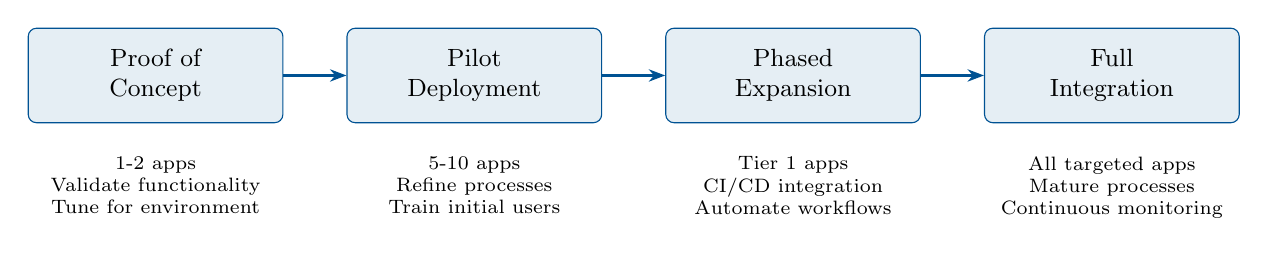
\begin{tikzpicture}[
    node distance=0.8cm,
    stepbox/.style={rectangle, draw=primaryblue, fill=primaryblue!10, rounded corners=3pt, text width=3cm, minimum height=1.2cm, align=center, font=\small},
    arrow/.style={-{Stealth[scale=0.9]}, thick, primaryblue}
]
    \node[stepbox] (poc) {Proof of\\Concept};
    \node[stepbox, right=of poc] (pilot) {Pilot\\Deployment};
    \node[stepbox, right=of pilot] (expand) {Phased\\Expansion};
    \node[stepbox, right=of expand] (full) {Full\\Integration};
    
    \draw[arrow] (poc) -- (pilot);
    \draw[arrow] (pilot) -- (expand);
    \draw[arrow] (expand) -- (full);
    
    \node[below=0.3cm of poc, font=\scriptsize, text width=3cm, align=center] {1-2 apps\\Validate functionality\\Tune for environment};
    \node[below=0.3cm of pilot, font=\scriptsize, text width=3cm, align=center] {5-10 apps\\Refine processes\\Train initial users};
    \node[below=0.3cm of expand, font=\scriptsize, text width=3cm, align=center] {Tier 1 apps\\CI/CD integration\\Automate workflows};
    \node[below=0.3cm of full, font=\scriptsize, text width=3cm, align=center] {All targeted apps\\Mature processes\\Continuous monitoring};
\end{tikzpicture}
\caption{Tool Deployment Progression}
\label{fig:tool-deployment}
\end{figure}

\clearpage
\subsection{Vulnerability Management Foundation}

\subsubsection{Tracking System Implementation}

Establish the vulnerability tracking system as the central repository for all security findings:

\begin{table}[H]
\centering
\renewcommand{\arraystretch}{1.3}
\begin{tabularx}{\textwidth}{>{\bfseries}p{3cm} X}
\toprule
\textbf{Capability} & \textbf{Implementation Requirements} \\
\midrule
Finding Ingestion & Automated import from SAST, SCA, DAST tools; manual finding entry; API for custom integrations \\
Deduplication & Rules for identifying duplicate findings across tools and scans; consolidation logic \\
Severity Assignment & Consistent severity classification aligned with policy; support for environmental factors \\
Assignment Workflow & Automatic routing to responsible teams; escalation rules; SLA tracking \\
Status Tracking & Finding lifecycle states (new, confirmed, in-progress, resolved, accepted); verification workflow \\
Reporting & Dashboard views; trend analysis; SLA compliance; aging reports; export capabilities \\
Integration & Bidirectional sync with ticketing systems; notification integrations; CI/CD pipeline hooks \\
\bottomrule
\end{tabularx}
\caption{Vulnerability Tracking System Requirements}
\label{tab:vuln-tracking}
\end{table}

\subsubsection{Initial SLA Framework}

Define remediation SLAs that are achievable given current capabilities while establishing expectations for improvement:

\begin{table}[H]
\centering
\renewcommand{\arraystretch}{1.3}
\begin{tabularx}{\textwidth}{>{\bfseries\centering\arraybackslash}p{2cm} >{\centering\arraybackslash}p{2.5cm} >{\centering\arraybackslash}p{2.5cm} X}
\toprule
\textbf{Severity} & \textbf{Phase 1 SLA} & \textbf{Target SLA} & \textbf{Notes} \\
\midrule
Critical & 7 days & 24-72 hours & Expedited process for actively exploited \\
High & 30 days & 14 days & Prioritized remediation \\
Medium & 90 days & 60 days & Scheduled maintenance \\
Low & 180 days & 90 days & Normal release cycle \\
\bottomrule
\end{tabularx}
\caption{Phase 1 Remediation SLAs}
\label{tab:phase1-slas}
\end{table}

\clearpage
\subsection{Training and Awareness}

\subsubsection{Awareness Program Launch}

Launch security awareness activities targeting all development personnel:

\begin{table}[H]
\centering
\renewcommand{\arraystretch}{1.3}
\begin{tabularx}{\textwidth}{>{\bfseries}p{3cm} p{3cm} X}
\toprule
\textbf{Activity} & \textbf{Target Audience} & \textbf{Content Focus} \\
\midrule
Program Announcement & All engineering & Program overview; vision and goals; how to engage \\
Security Newsletter & All engineering & Monthly security tips; threat updates; success stories \\
Lunch \& Learn Series & Development teams & Common vulnerabilities; secure coding basics; tool usage \\
OWASP Top 10 Overview & All developers & Awareness of most critical web application security risks \\
Tool Training & Initial tool users & Tool-specific training for SAST, SCA, tracking system \\
\bottomrule
\end{tabularx}
\caption{Phase 1 Awareness Activities}
\label{tab:phase1-awareness}
\end{table}

\subsubsection{Foundational Training Curriculum}

Develop and deploy foundational security training:

\begin{policybox}[Foundational Training Requirements]
\textbf{All Developers (Mandatory):}
\begin{itemize}[leftmargin=1.5em, itemsep=0.1em]
    \item Secure coding fundamentals (4 hours)
    \item OWASP Top 10 awareness (2 hours)
    \item Security tool usage basics (2 hours)
    \item Vulnerability remediation procedures (1 hour)
\end{itemize}

\textbf{Security Champions (Additional):}
\begin{itemize}[leftmargin=1.5em, itemsep=0.1em]
    \item Advanced secure coding (8 hours)
    \item Threat modeling fundamentals (4 hours)
    \item Security testing overview (4 hours)
    \item Champion role and responsibilities (2 hours)
\end{itemize}

\textbf{Architects/Tech Leads (Additional):}
\begin{itemize}[leftmargin=1.5em, itemsep=0.1em]
    \item Security architecture principles (4 hours)
    \item Threat modeling workshop (8 hours)
    \item Security requirements development (2 hours)
\end{itemize}
\end{policybox}

\clearpage
\subsection{Quick Wins}

Identify and execute quick wins that deliver visible value early in the program:

\begin{examplebox}[Phase 1 Quick Win Opportunities]
\begin{itemize}[leftmargin=1.5em, itemsep=0.3em]
    \item \textbf{Secrets Scanning:} Deploy pre-commit hooks to prevent credential leakage---immediate, high-visibility impact
    \item \textbf{Critical Vulnerability Remediation:} Address any known critical vulnerabilities in Tier 1 applications
    \item \textbf{Dependency Updates:} Update severely outdated components with known critical CVEs
    \item \textbf{Security Headers:} Implement standard security headers across web applications
    \item \textbf{HTTPS Enforcement:} Ensure all public-facing applications use HTTPS exclusively
    \item \textbf{Default Credential Removal:} Identify and remediate default credentials in test/production environments
    \item \textbf{Error Handling Review:} Address applications exposing sensitive information in error messages
\end{itemize}
\end{examplebox}

\subsection{Phase 1 Milestones and Deliverables}

\begin{milestonebox}[Phase 1 Milestone Summary]
\textbf{Month 2 Milestones:}
\begin{itemize}[leftmargin=1.5em, itemsep=0.1em]
    \item Executive sponsor confirmed with signed charter
    \item Steering committee formed with first meeting completed
    \item Program manager assigned and announced
    \item Vulnerability tracking system deployed and operational
    \item Secrets scanning deployed organization-wide
\end{itemize}

\textbf{Month 4 Milestones:}
\begin{itemize}[leftmargin=1.5em, itemsep=0.1em]
    \item Core security policies approved
    \item SAST deployed for Tier 1 applications
    \item SCA deployed for Tier 1 applications
    \item Initial Security Champions identified and onboarded
    \item Foundational training content developed
\end{itemize}

\textbf{Month 6 Milestones:}
\begin{itemize}[leftmargin=1.5em, itemsep=0.1em]
    \item All Tier 1 applications under active security testing
    \item Vulnerability management process operational with SLA tracking
    \item First executive dashboard delivered
    \item 50\% of developers completed foundational training
    \item DAST proof of concept completed
    \item Phase 2 plan approved
\end{itemize}
\end{milestonebox}

\subsection{Phase 1 Success Criteria}

\begin{table}[H]
\centering
\renewcommand{\arraystretch}{1.3}
\begin{tabularx}{\textwidth}{>{\bfseries}p{4cm} X >{\centering\arraybackslash}p{2.5cm}}
\toprule
\textbf{Success Criterion} & \textbf{Measurement Method} & \textbf{Target} \\
\midrule
Governance Established & Charter signed; committee active; policies approved & 100\% complete \\
Tier 1 Coverage & Tier 1 apps with SAST and SCA deployed & 100\% \\
Tool Integration & Tier 1 apps with CI/CD integration & $\geq$75\% \\
Vulnerability Tracking & Active findings tracked in central system & 100\% \\
Training Completion & Developers completing foundational training & $\geq$50\% \\
Champion Network & Security Champions active and trained & $\geq$1 per major team \\
Remediation SLA & Critical/High findings remediated within SLA & $\geq$70\% \\
Executive Reporting & Monthly reports delivered to steering committee & 100\% \\
\bottomrule
\end{tabularx}
\caption{Phase 1 Success Criteria}
\label{tab:phase1-success}
\end{table}

% ============================================================================
% SECTION 4: PHASE 2 - CORE BUILD
% ============================================================================
\clearpage
\section{Phase 2: Core Build (Months 7-12)}

Phase 2 builds upon the foundation established in Phase 1, expanding security testing coverage, deepening CI/CD integration, and maturing vulnerability management processes. This phase focuses on establishing consistent, repeatable security practices across the development organization.

\begin{phasebox}[Phase 2 Overview]{phase2}
\textbf{Duration:} 6 months (Months 7-12)\\
\textbf{Target Maturity:} Level 2 $\rightarrow$ Level 3\\
\textbf{Primary Focus:} Testing expansion, CI/CD integration, process standardization\\
\textbf{Key Outcomes:} Tier 1-2 coverage, automated gates, threat modeling, training completion
\end{phasebox}

\subsection{Phase 2 Objectives}

\begin{enumerate}[leftmargin=2em, itemsep=0.4em]
    \item Extend security testing coverage to all Tier 1 and Tier 2 applications
    \item Achieve full CI/CD integration with automated security gates
    \item Deploy DAST capabilities for production and pre-production testing
    \item Establish threat modeling practice for new projects and major changes
    \item Complete foundational security training for all development personnel
    \item Implement security metrics dashboard with trend analysis
    \item Mature vulnerability management with improved SLA compliance
    \item Expand Security Champion program to all major development teams
\end{enumerate}

\clearpage
\subsection{Testing Program Expansion}

\subsubsection{Coverage Expansion}

\begin{table}[H]
\centering
\renewcommand{\arraystretch}{1.3}
\begin{tabularx}{\textwidth}{>{\bfseries}p{2.5cm} p{3cm} p{3cm} X}
\toprule
\textbf{Tool Category} & \textbf{Phase 1 Coverage} & \textbf{Phase 2 Target} & \textbf{Key Activities} \\
\midrule
SAST & Tier 1 apps & Tier 1-2 apps (100\%) & Language expansion; custom rule development; tuning \\
SCA & Tier 1 apps & Tier 1-2 apps (100\%) & License compliance; continuous monitoring; SBOM generation \\
DAST & POC complete & Tier 1 apps (100\%) & Full deployment; authenticated scanning; API testing \\
Secrets Scanning & All repos & All repos + enhanced & Pre-commit enforcement; historical scanning; remediation \\
Container Scanning & Not started & Tier 1 containers & Image scanning; registry integration; policy enforcement \\
\bottomrule
\end{tabularx}
\caption{Phase 2 Testing Coverage Expansion}
\label{tab:phase2-coverage}
\end{table}

\subsubsection{CI/CD Integration Deepening}

Achieve comprehensive CI/CD integration with automated security gates:

\begin{figure}[H]
\centering
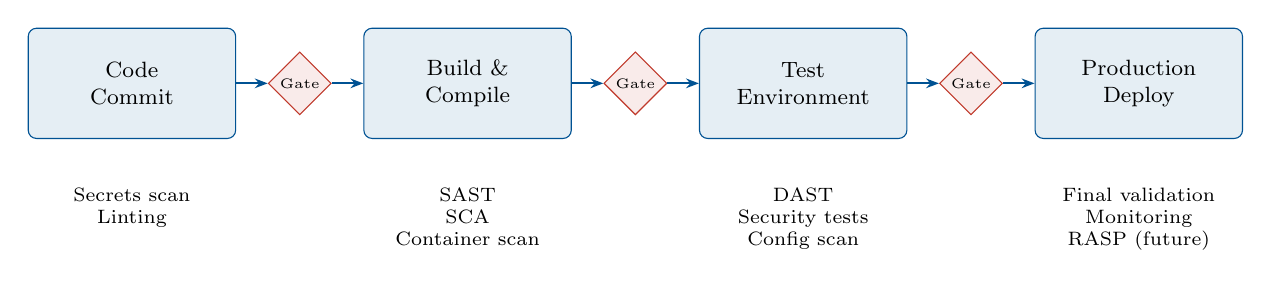
\begin{tikzpicture}[
    node distance=0.4cm,
    stage/.style={rectangle, draw=primaryblue, fill=primaryblue!10, rounded corners=3pt, text width=2.4cm, minimum height=1.4cm, align=center, font=\footnotesize},
    gate/.style={diamond, draw=alertred, fill=alertred!10, minimum width=0.8cm, minimum height=0.8cm, font=\tiny, inner sep=1pt},
    arrow/.style={-{Stealth[scale=0.7]}, thick, primaryblue}
]
    % Pipeline stages
    \node[stage] (commit) {Code\\Commit};
    \node[gate, right=of commit] (g1) {Gate};
    \node[stage, right=of g1] (build) {Build \&\\Compile};
    \node[gate, right=of build] (g2) {Gate};
    \node[stage, right=of g2] (test) {Test\\Environment};
    \node[gate, right=of test] (g3) {Gate};
    \node[stage, right=of g3] (deploy) {Production\\Deploy};
    
    % Arrows
    \draw[arrow] (commit) -- (g1);
    \draw[arrow] (g1) -- (build);
    \draw[arrow] (build) -- (g2);
    \draw[arrow] (g2) -- (test);
    \draw[arrow] (test) -- (g3);
    \draw[arrow] (g3) -- (deploy);
    
    % Security activities below
    \node[below=0.5cm of commit, font=\scriptsize, text width=2.4cm, align=center] {Secrets scan\\Linting};
    \node[below=0.5cm of build, font=\scriptsize, text width=2.4cm, align=center] {SAST\\SCA\\Container scan};
    \node[below=0.5cm of test, font=\scriptsize, text width=2.4cm, align=center] {DAST\\Security tests\\Config scan};
    \node[below=0.5cm of deploy, font=\scriptsize, text width=2.4cm, align=center] {Final validation\\Monitoring\\RASP (future)};
\end{tikzpicture}
\caption{Integrated Security Pipeline}
\label{fig:security-pipeline}
\end{figure}

\clearpage
\subsubsection{Security Gate Criteria}

Define explicit criteria for automated security gates:

\begin{table}[H]
\centering
\renewcommand{\arraystretch}{1.3}
\begin{tabularx}{\textwidth}{>{\bfseries}p{2.5cm} X X}
\toprule
\textbf{Gate} & \textbf{Blocking Criteria} & \textbf{Warning Criteria} \\
\midrule
Pre-Commit & Secrets detected; critical linting violations & High-severity linting issues \\
Build & Critical SAST findings; critical SCA vulnerabilities; base image with critical CVEs & High SAST/SCA findings; outdated dependencies \\
Pre-Deploy & Any unresolved critical/high from build; DAST critical findings; failed security tests & Medium findings above threshold; configuration drift \\
Production & All previous gates passed; required approvals obtained & Documentation gaps; monitoring not confirmed \\
\bottomrule
\end{tabularx}
\caption{Security Gate Criteria}
\label{tab:gate-criteria}
\end{table}

\clearpage
\subsection{Threat Modeling Implementation}

\subsubsection{Threat Modeling Program}

Establish threat modeling as a standard practice for new development and significant changes:

\begin{table}[H]
\centering
\renewcommand{\arraystretch}{1.3}
\begin{tabularx}{\textwidth}{>{\bfseries}p{3cm} X}
\toprule
\textbf{Component} & \textbf{Implementation Details} \\
\midrule
Methodology Selection & Select and standardize on a methodology (STRIDE, PASTA, Attack Trees); develop templates and guidance \\
Trigger Criteria & Define when threat modeling is required: new applications, major changes, new data flows, architecture changes \\
Facilitation Model & Train security team members as facilitators; develop workshop format; create self-service option for lower-tier apps \\
Tool Support & Evaluate and deploy threat modeling tools; integrate with architecture documentation systems \\
Quality Review & Establish review process for completed threat models; track identified threats through remediation \\
Training & Include threat modeling in Security Champion curriculum; offer workshops for architects and tech leads \\
\bottomrule
\end{tabularx}
\caption{Threat Modeling Program Components}
\label{tab:threat-modeling}
\end{table}

\subsubsection{Threat Modeling Rollout}

\begin{examplebox}[Threat Modeling Rollout Schedule]
\textbf{Month 7-8:}
\begin{itemize}[leftmargin=1.5em, itemsep=0.1em]
    \item Select methodology and develop templates
    \item Train initial facilitators (2-3 security team members)
    \item Conduct pilot threat models on 2-3 applications
\end{itemize}

\textbf{Month 9-10:}
\begin{itemize}[leftmargin=1.5em, itemsep=0.1em]
    \item Refine process based on pilot feedback
    \item Conduct threat modeling workshop for architects
    \item Begin requiring threat models for new Tier 1 projects
\end{itemize}

\textbf{Month 11-12:}
\begin{itemize}[leftmargin=1.5em, itemsep=0.1em]
    \item Extend requirement to Tier 2 new projects
    \item Complete threat models for existing Tier 1 applications
    \item Integrate threat model findings with vulnerability tracking
\end{itemize}
\end{examplebox}

\clearpage
\subsection{Vulnerability Management Maturation}

\subsubsection{Process Improvements}

\begin{table}[H]
\centering
\renewcommand{\arraystretch}{1.3}
\begin{tabularx}{\textwidth}{>{\bfseries}p{3cm} X X}
\toprule
\textbf{Process Area} & \textbf{Phase 1 State} & \textbf{Phase 2 Target} \\
\midrule
Triage & Manual triage; inconsistent severity assignment & Automated triage rules; environmental context; consistent severity \\
Prioritization & Ad-hoc prioritization & Risk-based prioritization considering exploitability, exposure, asset value \\
Assignment & Manual assignment & Automated routing based on code ownership; team workload balancing \\
Remediation & Developer-led with limited support & Remediation playbooks; security team consultation; code review support \\
Verification & Manual verification & Automated re-scan verification; regression test integration \\
Exception Mgmt & Informal exceptions & Formal exception workflow with approvals, compensating controls, expiration \\
\bottomrule
\end{tabularx}
\caption{Vulnerability Management Process Maturation}
\label{tab:vuln-mgmt-maturation}
\end{table}

\subsubsection{SLA Tightening}

Improve remediation SLAs as capabilities mature:

\begin{table}[H]
\centering
\renewcommand{\arraystretch}{1.3}
\begin{tabularx}{\textwidth}{>{\bfseries\centering\arraybackslash}p{2cm} >{\centering\arraybackslash}p{2.5cm} >{\centering\arraybackslash}p{2.5cm} >{\centering\arraybackslash}p{2.5cm} X}
\toprule
\textbf{Severity} & \textbf{Phase 1 SLA} & \textbf{Phase 2 SLA} & \textbf{Compliance Target} & \textbf{Escalation} \\
\midrule
Critical & 7 days & 72 hours & 95\% & Director at 24h \\
High & 30 days & 14 days & 90\% & Manager at 7d \\
Medium & 90 days & 45 days & 85\% & Lead at 30d \\
Low & 180 days & 90 days & 80\% & Quarterly review \\
\bottomrule
\end{tabularx}
\caption{Phase 2 Remediation SLAs}
\label{tab:phase2-slas}
\end{table}

\clearpage
\subsection{Metrics and Reporting Enhancement}

\subsubsection{Metrics Dashboard}

Deploy a comprehensive security metrics dashboard:

\begin{keyconceptbox}[Security Metrics Dashboard Components]
\textbf{Operational Metrics:}
\begin{itemize}[leftmargin=1.5em, itemsep=0.1em]
    \item Open vulnerabilities by severity, age, application, team
    \item Remediation rate trends (opened vs. closed over time)
    \item Mean time to remediation by severity
    \item SLA compliance percentage
    \item Security gate pass/fail rates
\end{itemize}

\textbf{Coverage Metrics:}
\begin{itemize}[leftmargin=1.5em, itemsep=0.1em]
    \item Applications under active testing by tier
    \item CI/CD integration percentage
    \item Training completion rates by team
    \item Threat model coverage for applicable projects
\end{itemize}

\textbf{Trend Analysis:}
\begin{itemize}[leftmargin=1.5em, itemsep=0.1em]
    \item Vulnerability density trends over time
    \item Recurring vulnerability patterns
    \item Team performance comparisons
    \item Risk posture trends by application tier
\end{itemize}
\end{keyconceptbox}

\clearpage
\subsection{Training Program Completion}

\subsubsection{Training Rollout Completion}

\begin{table}[H]
\centering
\renewcommand{\arraystretch}{1.3}
\begin{tabularx}{\textwidth}{>{\bfseries}p{3cm} >{\centering\arraybackslash}p{2cm} >{\centering\arraybackslash}p{2.5cm} X}
\toprule
\textbf{Training Module} & \textbf{Duration} & \textbf{Phase 2 Target} & \textbf{Delivery Method} \\
\midrule
Secure Coding Fundamentals & 4 hours & 100\% developers & E-learning + hands-on labs \\
OWASP Top 10 & 2 hours & 100\% developers & E-learning \\
Tool Usage (SAST/SCA) & 2 hours & Teams with coverage & Instructor-led workshop \\
Threat Modeling Basics & 4 hours & Champions + Architects & Workshop \\
Security Champion Advanced & 20 hours & All Champions & Blended learning \\
Language-Specific Security & 4 hours & Relevant developers & E-learning by language \\
\bottomrule
\end{tabularx}
\caption{Phase 2 Training Completion Targets}
\label{tab:phase2-training}
\end{table}

\subsection{Phase 2 Milestones and Deliverables}

\begin{milestonebox}[Phase 2 Milestone Summary]
\textbf{Month 8 Milestones:}
\begin{itemize}[leftmargin=1.5em, itemsep=0.1em]
    \item DAST fully deployed for Tier 1 applications
    \item All Tier 2 applications onboarded to SAST/SCA
    \item Threat modeling methodology selected and pilots completed
    \item Security metrics dashboard deployed
\end{itemize}

\textbf{Month 10 Milestones:}
\begin{itemize}[leftmargin=1.5em, itemsep=0.1em]
    \item CI/CD integration complete for Tier 1-2 applications
    \item Security gates enforced for Tier 1 applications
    \item 100\% of developers completed foundational training
    \item Container scanning deployed for Tier 1 containers
\end{itemize}

\textbf{Month 12 Milestones:}
\begin{itemize}[leftmargin=1.5em, itemsep=0.1em]
    \item 100\% Tier 1-2 applications under full testing coverage
    \item Threat models completed for all Tier 1 applications
    \item Security Champion in every major development team
    \item Phase 2 SLAs achieved with $\geq$85\% compliance
    \item Annual penetration test completed for Tier 1 applications
    \item Phase 3 plan approved
\end{itemize}
\end{milestonebox}

\subsection{Phase 2 Success Criteria}

\begin{table}[H]
\centering
\renewcommand{\arraystretch}{1.3}
\begin{tabularx}{\textwidth}{>{\bfseries}p{4cm} X >{\centering\arraybackslash}p{2.5cm}}
\toprule
\textbf{Success Criterion} & \textbf{Measurement Method} & \textbf{Target} \\
\midrule
Tier 1-2 Testing Coverage & Applications with SAST, SCA, DAST deployed & 100\% \\
CI/CD Integration & Tier 1-2 apps with automated security in pipeline & 100\% \\
Security Gates & Tier 1 apps with enforced security gates & 100\% \\
Training Completion & All developers completed foundational training & 100\% \\
Champion Coverage & Major teams with active Security Champion & 100\% \\
Threat Model Coverage & Tier 1 applications with completed threat model & 100\% \\
SLA Compliance & Critical/High findings within Phase 2 SLAs & $\geq$85\% \\
Vulnerability Reduction & Critical/High open findings vs. Phase 1 end & $\geq$25\% reduction \\
\bottomrule
\end{tabularx}
\caption{Phase 2 Success Criteria}
\label{tab:phase2-success}
\end{table}

% ============================================================================
% SECTION 5: PHASE 3 - EXPANSION
% ============================================================================
\clearpage
\section{Phase 3: Expansion (Year 2)}

Phase 3 extends mature security capabilities across the entire application portfolio while introducing advanced testing methodologies and deepening integration with development workflows. This phase achieves comprehensive coverage and establishes the organization at a consistently managed maturity level.

\begin{phasebox}[Phase 3 Overview]{phase3}
\textbf{Duration:} 12 months (Year 2)\\
\textbf{Target Maturity:} Level 3 (Defined)\\
\textbf{Primary Focus:} Portfolio-wide coverage, advanced testing, process standardization\\
\textbf{Key Outcomes:} Full portfolio coverage, IAST deployment, security architecture, compliance automation
\end{phasebox}

\subsection{Phase 3 Objectives}

\begin{enumerate}[leftmargin=2em, itemsep=0.4em]
    \item Extend security testing coverage to all Tier 3 applications
    \item Deploy Interactive Application Security Testing (IAST) for Tier 1 applications
    \item Establish formal security architecture review process
    \item Implement API security testing program
    \item Automate compliance evidence collection and reporting
    \item Develop comprehensive Software Bill of Materials (SBOM) program
    \item Implement security regression testing capabilities
    \item Establish continuous security monitoring for production applications
    \item Mature developer self-service security capabilities
\end{enumerate}

\clearpage
\subsection{Portfolio-Wide Coverage}

\subsubsection{Tier 3 Application Onboarding}

Extend security testing to Tier 3 applications with appropriate depth:

\begin{table}[H]
\centering
\renewcommand{\arraystretch}{1.3}
\begin{tabularx}{\textwidth}{>{\bfseries}p{2.5cm} p{3.5cm} X}
\toprule
\textbf{Testing Type} & \textbf{Tier 3 Requirement} & \textbf{Implementation Approach} \\
\midrule
SAST & Required & Automated scanning with standard policy; self-service for developers \\
SCA & Required & Continuous CVE monitoring; automated dependency updates where safe \\
DAST & Risk-based & Automated scanning for internet-facing; on-request for internal \\
Threat Modeling & Simplified & Self-service threat model checklist; full model for elevated risk \\
Penetration Testing & Not required & Available on-request for specific concerns \\
\bottomrule
\end{tabularx}
\caption{Tier 3 Testing Requirements}
\label{tab:tier3-requirements}
\end{table}

\subsubsection{Coverage Dashboard}

\begin{table}[H]
\centering
\renewcommand{\arraystretch}{1.3}
\begin{tabularx}{\textwidth}{>{\bfseries}p{2.5cm} >{\centering\arraybackslash}p{2cm} >{\centering\arraybackslash}p{2cm} >{\centering\arraybackslash}p{2cm} >{\centering\arraybackslash}p{2cm}}
\toprule
\textbf{Capability} & \textbf{Tier 1} & \textbf{Tier 2} & \textbf{Tier 3} & \textbf{Tier 4} \\
\midrule
SAST & 100\% & 100\% & 100\% & Best effort \\
SCA & 100\% & 100\% & 100\% & Best effort \\
DAST & 100\% & 100\% & Risk-based & On request \\
IAST & 100\% & Pilot & --- & --- \\
Pen Testing & Annual & Annual & Biennial & On request \\
Threat Model & 100\% & 100\% & Checklist & --- \\
\bottomrule
\end{tabularx}
\caption{End of Phase 3 Coverage Targets}
\label{tab:phase3-coverage-targets}
\end{table}

\clearpage
\subsection{Advanced Testing Capabilities}

\subsubsection{IAST Deployment}

Deploy Interactive Application Security Testing for highest-value applications:

\begin{table}[H]
\centering
\renewcommand{\arraystretch}{1.3}
\begin{tabularx}{\textwidth}{>{\bfseries}p{3cm} X}
\toprule
\textbf{Deployment Phase} & \textbf{Activities} \\
\midrule
Q1 Year 2 & Tool selection and procurement; architecture planning; agent deployment strategy \\
Q2 Year 2 & Pilot deployment on 3-5 Tier 1 applications; integration with test environments; tuning \\
Q3 Year 2 & Expand to all Tier 1 applications; refine alerting and remediation workflows \\
Q4 Year 2 & Begin Tier 2 pilots; optimize performance impact; mature integration \\
\bottomrule
\end{tabularx}
\caption{IAST Deployment Schedule}
\label{tab:iast-deployment}
\end{table}

\subsubsection{API Security Testing}

Establish dedicated API security testing capabilities:

\begin{keyconceptbox}[API Security Testing Program]
\textbf{Scope:}
\begin{itemize}[leftmargin=1.5em, itemsep=0.1em]
    \item All external-facing APIs
    \item Internal APIs processing sensitive data
    \item Third-party API integrations
\end{itemize}

\textbf{Testing Components:}
\begin{itemize}[leftmargin=1.5em, itemsep=0.1em]
    \item API specification review (OpenAPI/Swagger security analysis)
    \item Authentication and authorization testing
    \item Input validation and injection testing
    \item Rate limiting and abuse prevention verification
    \item Data exposure and sensitive data handling
    \item Business logic vulnerability testing
\end{itemize}

\textbf{Integration:}
\begin{itemize}[leftmargin=1.5em, itemsep=0.1em]
    \item Automated API security scanning in CI/CD
    \item API gateway security policy enforcement
    \item API inventory and discovery automation
\end{itemize}
\end{keyconceptbox}

\clearpage
\subsection{Security Architecture Program}

\subsubsection{Architecture Review Process}

Formalize security architecture review for new development:

\begin{table}[H]
\centering
\renewcommand{\arraystretch}{1.3}
\begin{tabularx}{\textwidth}{>{\bfseries}p{3cm} p{4cm} X}
\toprule
\textbf{Review Type} & \textbf{Trigger Criteria} & \textbf{Review Scope} \\
\midrule
Full Review & New Tier 1-2 applications; major architecture changes & Complete architecture assessment; threat model; security requirements \\
Focused Review & Tier 3 applications; moderate changes & Targeted review of high-risk components; abbreviated threat model \\
Self-Assessment & Minor changes; Tier 4 applications & Checklist-based self-assessment with security consultation available \\
Pattern Review & New technology adoption; reference architecture development & Evaluation for security implications; guidance development \\
\bottomrule
\end{tabularx}
\caption{Security Architecture Review Types}
\label{tab:arch-review-types}
\end{table}

\subsubsection{Secure Architecture Patterns}

Develop and maintain a library of secure architecture patterns:

\begin{examplebox}[Secure Architecture Pattern Library]
\textbf{Authentication Patterns:}
\begin{itemize}[leftmargin=1.5em, itemsep=0.1em]
    \item OAuth 2.0/OIDC integration patterns
    \item Multi-factor authentication implementation
    \item Service-to-service authentication
    \item API key and token management
\end{itemize}

\textbf{Data Protection Patterns:}
\begin{itemize}[leftmargin=1.5em, itemsep=0.1em]
    \item Encryption at rest implementation
    \item TLS/mTLS configuration
    \item Key management architecture
    \item Data classification and handling
\end{itemize}

\textbf{Application Patterns:}
\begin{itemize}[leftmargin=1.5em, itemsep=0.1em]
    \item Input validation and output encoding
    \item Session management
    \item Error handling and logging
    \item API gateway integration
\end{itemize}
\end{examplebox}

\clearpage
\subsection{Compliance Automation}

\subsubsection{Evidence Collection Automation}

Automate collection of compliance evidence to reduce audit burden:

\begin{table}[H]
\centering
\renewcommand{\arraystretch}{1.3}
\begin{tabularx}{\textwidth}{>{\bfseries}p{3cm} X X}
\toprule
\textbf{Control Area} & \textbf{Evidence Type} & \textbf{Automation Approach} \\
\midrule
Security Testing & Scan reports; coverage metrics; finding trends & Automated export from security tools; scheduled report generation \\
Vulnerability Mgmt & Open/closed findings; SLA compliance; exception logs & Dashboard snapshots; API-driven data extraction \\
Access Control & Permission reviews; access logs; provisioning records & Integration with identity systems; automated access reviews \\
Change Management & Deployment records; approval logs; rollback history & CI/CD pipeline logs; audit trail integration \\
Training & Completion rates; certification records; attendance logs & LMS integration; automated compliance reports \\
\bottomrule
\end{tabularx}
\caption{Compliance Evidence Automation}
\label{tab:compliance-automation}
\end{table}

\subsection{SBOM Program}

\subsubsection{Software Bill of Materials Implementation}

Establish comprehensive SBOM generation and management:

\begin{policybox}[SBOM Program Requirements]
\textbf{Generation:}
\begin{itemize}[leftmargin=1.5em, itemsep=0.1em]
    \item Automated SBOM generation during build process
    \item Standard format adoption (SPDX or CycloneDX)
    \item Complete component inventory including transitive dependencies
    \item Version and license information capture
\end{itemize}

\textbf{Management:}
\begin{itemize}[leftmargin=1.5em, itemsep=0.1em]
    \item Centralized SBOM repository with versioning
    \item Linkage to deployed application versions
    \item Searchable component database for vulnerability response
    \item Integration with SCA tools for continuous monitoring
\end{itemize}

\textbf{Usage:}
\begin{itemize}[leftmargin=1.5em, itemsep=0.1em]
    \item Rapid impact assessment for new CVE disclosures
    \item License compliance verification
    \item Supply chain risk analysis
    \item Customer/regulatory SBOM requests
\end{itemize}
\end{policybox}

\clearpage
\subsection{Phase 3 Milestones and Success Criteria}

\begin{milestonebox}[Phase 3 Milestone Summary]
\textbf{Q1 Year 2:}
\begin{itemize}[leftmargin=1.5em, itemsep=0.1em]
    \item Tier 3 onboarding plan finalized; first wave onboarded
    \item IAST pilot initiated
    \item Security architecture review process documented and launched
    \item SBOM generation integrated into build pipelines
\end{itemize}

\textbf{Q2 Year 2:}
\begin{itemize}[leftmargin=1.5em, itemsep=0.1em]
    \item 50\% Tier 3 applications onboarded
    \item API security testing program operational
    \item Compliance evidence automation implemented
    \item Security pattern library launched
\end{itemize}

\textbf{Q3 Year 2:}
\begin{itemize}[leftmargin=1.5em, itemsep=0.1em]
    \item IAST deployed for all Tier 1 applications
    \item 100\% Tier 3 applications onboarded
    \item Production security monitoring operational
    \item Developer self-service portal enhanced
\end{itemize}

\textbf{Q4 Year 2:}
\begin{itemize}[leftmargin=1.5em, itemsep=0.1em]
    \item Full portfolio coverage achieved
    \item IAST Tier 2 pilots initiated
    \item Annual program maturity assessment completed
    \item Phase 4 plan approved
\end{itemize}
\end{milestonebox}

\begin{table}[H]
\centering
\renewcommand{\arraystretch}{1.3}
\begin{tabularx}{\textwidth}{>{\bfseries}p{4cm} X >{\centering\arraybackslash}p{2.5cm}}
\toprule
\textbf{Success Criterion} & \textbf{Measurement} & \textbf{Target} \\
\midrule
Portfolio Coverage & Tier 1-3 apps with appropriate testing & 100\% \\
IAST Deployment & Tier 1 apps with IAST operational & 100\% \\
Architecture Reviews & New Tier 1-2 projects with security review & 100\% \\
SBOM Coverage & Applications with generated SBOMs & $\geq$90\% \\
API Security & External APIs under security testing & 100\% \\
SLA Compliance & Critical/High within SLA & $\geq$90\% \\
Training Currency & Developers with current training & $\geq$95\% \\
Maturity Level & BSIMM/SAMM assessment score & Level 3 \\
\bottomrule
\end{tabularx}
\caption{Phase 3 Success Criteria}
\label{tab:phase3-success}
\end{table}

% ============================================================================
% SECTION 6: PHASE 4 - OPTIMIZATION
% ============================================================================
\clearpage
\section{Phase 4: Optimization (Year 3)}

Phase 4 focuses on optimizing security operations, improving efficiency, enhancing developer experience, and advancing toward a quantitatively managed program. This phase transforms security from a defined practice into a well-managed discipline with predictable outcomes.

\begin{phasebox}[Phase 4 Overview]{phase4}
\textbf{Duration:} 12 months (Year 3)\\
\textbf{Target Maturity:} Level 3 $\rightarrow$ Level 4 (Managed)\\
\textbf{Primary Focus:} Process optimization, automation, predictive capabilities\\
\textbf{Key Outcomes:} Efficient operations, developer self-service, predictive analytics, reduced friction
\end{phasebox}

\subsection{Phase 4 Objectives}

\begin{enumerate}[leftmargin=2em, itemsep=0.4em]
    \item Optimize security testing for minimal developer friction
    \item Implement advanced automation for vulnerability management
    \item Deploy Runtime Application Self-Protection (RASP) for Tier 1 applications
    \item Establish security engineering platform for developer self-service
    \item Implement predictive security analytics
    \item Achieve consistent SLA performance with minimal exceptions
    \item Develop security gamification and incentive programs
    \item Establish security research and emerging threat capabilities
\end{enumerate}

\clearpage
\subsection{Developer Experience Optimization}

\subsubsection{Friction Reduction Initiatives}

\begin{table}[H]
\centering
\renewcommand{\arraystretch}{1.3}
\begin{tabularx}{\textwidth}{>{\bfseries}p{3cm} X X}
\toprule
\textbf{Friction Point} & \textbf{Optimization Approach} & \textbf{Success Metric} \\
\midrule
False Positives & Advanced tuning; context-aware rules; machine learning filtering & False positive rate $<$15\% \\
Scan Time & Incremental scanning; parallel execution; intelligent scheduling & Scan completes within build window \\
Remediation Clarity & Enhanced guidance; auto-fix suggestions; example code & Developer satisfaction $\geq$4/5 \\
Tool Access & Single sign-on; unified dashboard; mobile access & Onboarding time $<$30 minutes \\
Approval Delays & Automated approvals for low-risk; clear escalation & Gate approval $<$4 hours \\
\bottomrule
\end{tabularx}
\caption{Developer Friction Reduction Initiatives}
\label{tab:friction-reduction}
\end{table}

\subsubsection{Security Engineering Platform}

Develop a unified platform for developer security self-service:

\begin{keyconceptbox}[Security Engineering Platform Capabilities]
\textbf{Self-Service Security:}
\begin{itemize}[leftmargin=1.5em, itemsep=0.1em]
    \item On-demand security scans with instant results
    \item Threat modeling templates and guided workflows
    \item Security requirements generator based on project context
    \item Automated security design review for common patterns
\end{itemize}

\textbf{Remediation Support:}
\begin{itemize}[leftmargin=1.5em, itemsep=0.1em]
    \item Contextual remediation guidance within IDE
    \item Auto-fix capabilities for common vulnerability patterns
    \item Security code snippet library
    \item AI-assisted vulnerability explanation and fix suggestions
\end{itemize}

\textbf{Learning Integration:}
\begin{itemize}[leftmargin=1.5em, itemsep=0.1em]
    \item Just-in-time security training linked to findings
    \item Secure coding challenges and competitions
    \item Progress tracking and skill certification
    \item Peer learning and knowledge sharing
\end{itemize}
\end{keyconceptbox}

\clearpage
\subsection{Advanced Automation}

\subsubsection{Intelligent Vulnerability Management}

\begin{table}[H]
\centering
\renewcommand{\arraystretch}{1.3}
\begin{tabularx}{\textwidth}{>{\bfseries}p{3cm} X}
\toprule
\textbf{Capability} & \textbf{Implementation} \\
\midrule
Auto-Triage & Machine learning models for severity prediction; environmental context integration; exploitability assessment \\
Smart Routing & Automatic assignment based on code ownership, team capacity, expertise matching \\
Predictive SLA & Forecast SLA breaches; proactive escalation; workload balancing recommendations \\
Auto-Remediation & Automated dependency updates; configuration fixes; approved patch deployment \\
Duplicate Detection & Cross-tool deduplication; root cause grouping; finding consolidation \\
Risk Scoring & Real-time risk scoring incorporating threat intelligence, asset value, exposure \\
\bottomrule
\end{tabularx}
\caption{Intelligent Vulnerability Management Capabilities}
\label{tab:intelligent-vuln-mgmt}
\end{table}

\subsubsection{RASP Deployment}

Deploy Runtime Application Self-Protection for Tier 1 applications:

\begin{table}[H]
\centering
\renewcommand{\arraystretch}{1.3}
\begin{tabularx}{\textwidth}{>{\bfseries}p{2cm} X}
\toprule
\textbf{Phase} & \textbf{Activities} \\
\midrule
Q1 & Tool selection and procurement; architecture planning; performance baseline \\
Q2 & Pilot deployment (3 applications) in monitoring mode; alert tuning; integration testing \\
Q3 & Expand to all Tier 1 applications; enable blocking for validated attack patterns \\
Q4 & Optimize performance; mature operational procedures; begin Tier 2 planning \\
\bottomrule
\end{tabularx}
\caption{RASP Deployment Schedule}
\label{tab:rasp-deployment}
\end{table}

\clearpage
\subsection{Predictive Security Analytics}

\subsubsection{Analytics Capabilities}

\begin{examplebox}[Predictive Security Analytics Use Cases]
\textbf{Vulnerability Prediction:}
\begin{itemize}[leftmargin=1.5em, itemsep=0.1em]
    \item Identify code areas likely to contain vulnerabilities based on complexity, change frequency, developer patterns
    \item Predict vulnerability emergence based on dependency update patterns
    \item Forecast remediation capacity needs based on pipeline activity
\end{itemize}

\textbf{Risk Forecasting:}
\begin{itemize}[leftmargin=1.5em, itemsep=0.1em]
    \item Project security posture based on development roadmaps
    \item Anticipate compliance gaps before audit periods
    \item Model impact of architectural changes on risk profile
\end{itemize}

\textbf{Resource Optimization:}
\begin{itemize}[leftmargin=1.5em, itemsep=0.1em]
    \item Optimize testing resource allocation based on risk and coverage
    \item Predict staffing needs based on portfolio growth
    \item Identify high-impact training investments
\end{itemize}
\end{examplebox}

\subsection{Gamification and Incentives}

\subsubsection{Security Culture Enhancement}

\begin{table}[H]
\centering
\renewcommand{\arraystretch}{1.3}
\begin{tabularx}{\textwidth}{>{\bfseries}p{3cm} X X}
\toprule
\textbf{Program Element} & \textbf{Description} & \textbf{Recognition} \\
\midrule
Secure Code Leaderboard & Team rankings based on vulnerability density trends & Monthly recognition; quarterly prizes \\
Bug Bash Events & Focused security testing competitions & Awards; public recognition \\
Champion of the Month & Outstanding Security Champion contributions & Executive recognition; swag \\
Training Achievements & Completion of advanced security certifications & Badging; career advancement credit \\
Innovation Awards & Novel security solutions or improvements & Bonus; conference attendance \\
\bottomrule
\end{tabularx}
\caption{Security Gamification Programs}
\label{tab:gamification}
\end{table}

\clearpage
\subsection{Phase 4 Milestones and Success Criteria}

\begin{milestonebox}[Phase 4 Milestone Summary]
\textbf{Q1 Year 3:}
\begin{itemize}[leftmargin=1.5em, itemsep=0.1em]
    \item Developer friction assessment completed; top issues identified
    \item RASP pilot initiated
    \item Security engineering platform design approved
    \item Predictive analytics prototype developed
\end{itemize}

\textbf{Q2 Year 3:}
\begin{itemize}[leftmargin=1.5em, itemsep=0.1em]
    \item Auto-remediation operational for dependency updates
    \item Security platform MVP launched
    \item False positive rate reduced by 50\%
    \item Gamification program launched
\end{itemize}

\textbf{Q3 Year 3:}
\begin{itemize}[leftmargin=1.5em, itemsep=0.1em]
    \item RASP deployed for all Tier 1 applications
    \item Intelligent triage operational
    \item IDE security integration enhanced
    \item SLA compliance $\geq$95\%
\end{itemize}

\textbf{Q4 Year 3:}
\begin{itemize}[leftmargin=1.5em, itemsep=0.1em]
    \item Full security platform operational
    \item Predictive analytics in production
    \item Developer satisfaction $\geq$4/5
    \item Level 4 maturity assessment initiated
\end{itemize}
\end{milestonebox}

\begin{table}[H]
\centering
\renewcommand{\arraystretch}{1.3}
\begin{tabularx}{\textwidth}{>{\bfseries}p{4cm} X >{\centering\arraybackslash}p{2.5cm}}
\toprule
\textbf{Success Criterion} & \textbf{Measurement} & \textbf{Target} \\
\midrule
False Positive Rate & Verified FP percentage across all tools & $<$15\% \\
Developer Satisfaction & Annual security tools survey score & $\geq$4.0/5.0 \\
SLA Compliance & Critical/High findings within SLA & $\geq$95\% \\
Auto-Remediation Rate & Vulnerabilities auto-fixed without manual intervention & $\geq$30\% \\
RASP Coverage & Tier 1 applications with RASP deployed & 100\% \\
Platform Adoption & Developers actively using security platform & $\geq$80\% \\
Prediction Accuracy & Vulnerability prediction model accuracy & $\geq$75\% \\
Maturity Level & BSIMM/SAMM assessment score & Level 4 \\
\bottomrule
\end{tabularx}
\caption{Phase 4 Success Criteria}
\label{tab:phase4-success}
\end{table}

% ============================================================================
% SECTION 7: PHASE 5 - EXCELLENCE
% ============================================================================
\clearpage
\section{Phase 5: Excellence (Ongoing)}

Phase 5 represents the ongoing journey toward security excellence, focusing on continuous improvement, innovation, and maintaining industry leadership. This phase never truly ends but establishes the practices and culture necessary for sustained security excellence.

\begin{phasebox}[Phase 5 Overview]{phase5}
\textbf{Duration:} Ongoing (Year 4+)\\
\textbf{Target Maturity:} Level 4+ (Optimizing)\\
\textbf{Primary Focus:} Continuous improvement, innovation, industry leadership\\
\textbf{Key Outcomes:} Sustained excellence, adaptive capabilities, security innovation
\end{phasebox}

\subsection{Phase 5 Objectives}

\begin{enumerate}[leftmargin=2em, itemsep=0.4em]
    \item Establish continuous improvement processes with measurable outcomes
    \item Develop advanced threat intelligence and proactive security capabilities
    \item Achieve and maintain industry-leading security practices
    \item Foster security innovation and emerging technology adoption
    \item Build security thought leadership through community engagement
    \item Maintain adaptive capabilities for evolving threat landscapes
    \item Optimize return on security investment through ongoing efficiency gains
\end{enumerate}

\clearpage
\subsection{Continuous Improvement Framework}

\subsubsection{Improvement Cycle}

\begin{figure}[H]
\centering
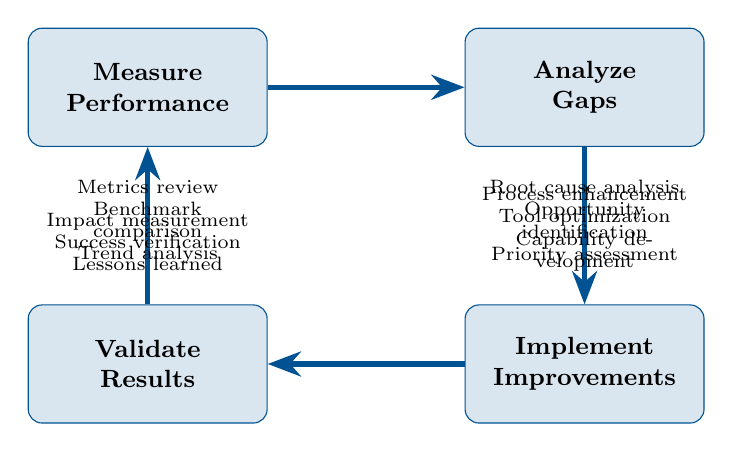
\begin{tikzpicture}[
    node distance=2.5cm,
    cycle/.style={rectangle, draw=primaryblue, fill=primaryblue!15, rounded corners=5pt, text width=2.8cm, minimum height=1.5cm, align=center, font=\small\bfseries},
    arrow/.style={-{Stealth[scale=1]}, thick, primaryblue, line width=2pt}
]
    \node[cycle] (measure) {Measure\\Performance};
    \node[cycle, right=of measure] (analyze) {Analyze\\Gaps};
    \node[cycle, below=2cm of analyze] (improve) {Implement\\Improvements};
    \node[cycle, left=of improve] (validate) {Validate\\Results};
    
    \draw[arrow] (measure) -- (analyze);
    \draw[arrow] (analyze) -- (improve);
    \draw[arrow] (improve) -- (validate);
    \draw[arrow] (validate) -- (measure);
    
    \node[below=0.3cm of measure, font=\scriptsize, text width=2.8cm, align=center] {Metrics review\\Benchmark comparison\\Trend analysis};
    \node[below=0.3cm of analyze, font=\scriptsize, text width=2.8cm, align=center] {Root cause analysis\\Opportunity identification\\Priority assessment};
    \node[above=0.3cm of improve, font=\scriptsize, text width=2.8cm, align=center] {Process enhancement\\Tool optimization\\Capability development};
    \node[above=0.3cm of validate, font=\scriptsize, text width=2.8cm, align=center] {Impact measurement\\Success verification\\Lessons learned};
\end{tikzpicture}
\caption{Continuous Improvement Cycle}
\label{fig:improvement-cycle}
\end{figure}

\subsubsection{Improvement Areas}

\begin{table}[H]
\centering
\renewcommand{\arraystretch}{1.3}
\begin{tabularx}{\textwidth}{>{\bfseries}p{3cm} X X}
\toprule
\textbf{Improvement Area} & \textbf{Focus} & \textbf{Cadence} \\
\midrule
Process Efficiency & Reduce cycle times; eliminate waste; streamline workflows & Quarterly review \\
Tool Optimization & Enhance accuracy; reduce false positives; improve integration & Monthly tuning \\
Coverage Expansion & Address gaps; new technology support; emerging architectures & Continuous assessment \\
Developer Experience & Reduce friction; improve satisfaction; enhance self-service & Bi-annual survey \\
Risk Reduction & Lower vulnerability density; faster remediation; reduced exposure & Monthly tracking \\
Cost Efficiency & Optimize spend; maximize ROI; consolidate tools & Annual review \\
\bottomrule
\end{tabularx}
\caption{Continuous Improvement Focus Areas}
\label{tab:improvement-areas}
\end{table}

\clearpage
\subsection{Advanced Threat Intelligence}

\subsubsection{Proactive Security Capabilities}

\begin{keyconceptbox}[Advanced Threat Intelligence Program]
\textbf{Threat Monitoring:}
\begin{itemize}[leftmargin=1.5em, itemsep=0.1em]
    \item Continuous monitoring of threat intelligence feeds
    \item Industry-specific threat tracking
    \item Emerging vulnerability trend analysis
    \item Attack technique evolution monitoring
\end{itemize}

\textbf{Proactive Response:}
\begin{itemize}[leftmargin=1.5em, itemsep=0.1em]
    \item Pre-emptive control enhancement for emerging threats
    \item Rapid response playbooks for zero-day scenarios
    \item Threat hunting integration with application telemetry
    \item Red team exercises informed by current threat landscape
\end{itemize}

\textbf{Intelligence Sharing:}
\begin{itemize}[leftmargin=1.5em, itemsep=0.1em]
    \item Participation in industry sharing organizations (ISACs)
    \item Internal threat briefings for development teams
    \item Security bulletin program for critical threats
    \item Vendor security coordination for disclosed vulnerabilities
\end{itemize}
\end{keyconceptbox}

\subsection{Innovation and Emerging Technology}

\subsubsection{Security Innovation Program}

\begin{table}[H]
\centering
\renewcommand{\arraystretch}{1.3}
\begin{tabularx}{\textwidth}{>{\bfseries}p{3cm} X}
\toprule
\textbf{Innovation Area} & \textbf{Activities} \\
\midrule
Emerging Tech Evaluation & Continuous evaluation of new security technologies; proof of concept programs; adoption recommendations \\
Research Partnerships & Academic partnerships; vendor beta programs; open source contributions \\
Internal Innovation & Hackathons; innovation time allocation; security research projects \\
AI/ML Security & Application of AI/ML to security challenges; adversarial ML defense; AI-generated code security \\
\bottomrule
\end{tabularx}
\caption{Security Innovation Program Components}
\label{tab:innovation-program}
\end{table}

\clearpage
\subsection{Industry Leadership}

\subsubsection{Thought Leadership Activities}

\begin{examplebox}[Security Thought Leadership Program]
\textbf{External Engagement:}
\begin{itemize}[leftmargin=1.5em, itemsep=0.1em]
    \item Conference presentations sharing lessons learned
    \item Blog posts and white papers on security practices
    \item Participation in standards development (OWASP, NIST)
    \item Open source security tool contributions
\end{itemize}

\textbf{Benchmarking:}
\begin{itemize}[leftmargin=1.5em, itemsep=0.1em]
    \item Annual BSIMM/SAMM assessment participation
    \item Industry peer benchmarking
    \item Third-party program assessments
    \item Certification maintenance (SOC 2, ISO 27001)
\end{itemize}

\textbf{Community Building:}
\begin{itemize}[leftmargin=1.5em, itemsep=0.1em]
    \item Host security meetups and events
    \item Mentorship programs for emerging security professionals
    \item University partnership and internship programs
    \item Customer security advisory relationships
\end{itemize}
\end{examplebox}

\subsection{Sustained Excellence Metrics}

\begin{table}[H]
\centering
\renewcommand{\arraystretch}{1.3}
\begin{tabularx}{\textwidth}{>{\bfseries}p{4cm} X >{\centering\arraybackslash}p{2.5cm}}
\toprule
\textbf{Excellence Indicator} & \textbf{Measurement} & \textbf{Target} \\
\midrule
Maturity Level & Annual BSIMM/SAMM assessment & Maintain Level 4+ \\
Vulnerability Density & Findings per 1000 lines of code & Year-over-year improvement \\
Time to Remediation & Mean time to fix critical vulnerabilities & $<$48 hours \\
Security Incidents & Application security-related incidents & Zero critical incidents \\
Developer Satisfaction & Annual security program survey & $\geq$4.5/5.0 \\
Coverage Completeness & Portfolio under appropriate testing & $>$98\% \\
Compliance Posture & Audit findings and deficiencies & Zero critical findings \\
Innovation Adoption & New capabilities implemented annually & $\geq$3 major initiatives \\
\bottomrule
\end{tabularx}
\caption{Sustained Excellence Metrics}
\label{tab:excellence-metrics}
\end{table}

% ============================================================================
% SECTION 8: RESOURCE REQUIREMENTS
% ============================================================================
\clearpage
\section{Resource Requirements}

Successful roadmap execution requires appropriate investment in personnel, tooling, and operational budget. This section provides guidance on resource planning across all phases.

\subsection{Staffing Requirements}

\subsubsection{Team Growth Trajectory}

\begin{table}[H]
\centering
\renewcommand{\arraystretch}{1.3}
\begin{tabularx}{\textwidth}{>{\bfseries}p{4cm} >{\centering\arraybackslash}p{1.8cm} >{\centering\arraybackslash}p{1.8cm} >{\centering\arraybackslash}p{1.8cm} >{\centering\arraybackslash}p{1.8cm} >{\centering\arraybackslash}p{1.8cm}}
\toprule
\textbf{Role} & \textbf{Phase 1} & \textbf{Phase 2} & \textbf{Phase 3} & \textbf{Phase 4} & \textbf{Phase 5} \\
\midrule
Program Manager & 1.0 & 1.0 & 1.0 & 1.0 & 1.0 \\
Security Architects & 0.5--1.0 & 1.0 & 1.5--2.0 & 2.0 & 2.0 \\
Security Engineers & 1.0--2.0 & 2.0--3.0 & 3.0--4.0 & 4.0--5.0 & 4.0--5.0 \\
Security Analysts & 1.0--2.0 & 2.0--3.0 & 3.0--4.0 & 3.0--4.0 & 3.0--4.0 \\
Training Specialist & 0.5 & 1.0 & 1.0 & 1.0 & 1.0 \\
Penetration Testers & 0 & 1.0--2.0 & 2.0--3.0 & 2.0--3.0 & 2.0--3.0 \\
\midrule
\textbf{Total FTE} & \textbf{4--6.5} & \textbf{8--12} & \textbf{12--16} & \textbf{13--17} & \textbf{13--17} \\
\bottomrule
\end{tabularx}
\caption{Application Security Team Staffing by Phase}
\label{tab:staffing-phases}
\end{table}

\begin{notebox}[Staffing Guidance]
Staffing requirements scale with application portfolio size and complexity. The figures above assume a medium-sized enterprise with 100-300 applications. Organizations should adjust based on:
\begin{itemize}[leftmargin=1.5em, itemsep=0.1em]
    \item Total application count
    \item Proportion of high-risk applications
    \item Development team size and velocity
    \item Regulatory complexity
    \item In-house vs. outsourced development mix
\end{itemize}
A common benchmark is 1 security FTE per 100 developers for mature programs.
\end{notebox}

\subsubsection{Security Champion Allocation}

\begin{table}[H]
\centering
\renewcommand{\arraystretch}{1.3}
\begin{tabularx}{\textwidth}{>{\bfseries}p{3cm} >{\centering\arraybackslash}p{2cm} >{\centering\arraybackslash}p{2cm} X}
\toprule
\textbf{Phase} & \textbf{Champions} & \textbf{Time Allocation} & \textbf{Coverage Target} \\
\midrule
Phase 1 & 5--10 & 10\% & 1 per Tier 1 application team \\
Phase 2 & 15--25 & 15\% & 1 per major development team \\
Phase 3 & 25--40 & 15\% & 1 per development team \\
Phase 4+ & 30--50 & 15--20\% & 1 per 8--10 developers \\
\bottomrule
\end{tabularx}
\caption{Security Champion Program Scaling}
\label{tab:champion-scaling}
\end{table}

\subsection{Tooling Budget}

\subsubsection{Tool Investment by Phase}

\begin{table}[H]
\centering
\renewcommand{\arraystretch}{1.3}
\begin{tabularx}{\textwidth}{>{\bfseries}p{3.5cm} >{\centering\arraybackslash}p{2cm} >{\centering\arraybackslash}p{2cm} >{\centering\arraybackslash}p{2cm} >{\centering\arraybackslash}p{2cm}}
\toprule
\textbf{Tool Category} & \textbf{Phase 1} & \textbf{Phase 2} & \textbf{Phase 3} & \textbf{Phase 4} \\
\midrule
SAST & \$\$\$ & --- & Expansion & Optimization \\
SCA & \$\$\$ & --- & Expansion & Optimization \\
DAST & Pilot & \$\$\$ & Expansion & Optimization \\
Secrets Scanning & \$\$ & --- & --- & --- \\
Vulnerability Management & \$\$\$ & --- & Expansion & --- \\
IAST & --- & --- & \$\$\$ & --- \\
RASP & --- & --- & Pilot & \$\$\$ \\
Container Security & --- & \$\$ & Expansion & --- \\
API Security & --- & --- & \$\$ & Expansion \\
Security Platform & --- & --- & \$\$ & \$\$\$ \\
\midrule
\textbf{Annual Range} & \$200--400K & \$150--300K & \$200--400K & \$150--300K \\
\bottomrule
\end{tabularx}
\caption{Tool Investment by Phase (Illustrative)}
\label{tab:tool-investment}
\end{table}

\begin{notebox}[Tool Budget Considerations]
Actual tool costs vary significantly based on:
\begin{itemize}[leftmargin=1.5em, itemsep=0.1em]
    \item Vendor selection (commercial vs. open source)
    \item Licensing model (per-user, per-application, per-scan)
    \item Portfolio size and growth rate
    \item Negotiated enterprise agreements
    \item Existing tool investments that can be leveraged
\end{itemize}
\end{notebox}

\subsection{Operational Budget}

\begin{table}[H]
\centering
\renewcommand{\arraystretch}{1.3}
\begin{tabularx}{\textwidth}{>{\bfseries}p{4cm} X >{\centering\arraybackslash}p{2.5cm}}
\toprule
\textbf{Budget Category} & \textbf{Components} & \textbf{Annual Estimate} \\
\midrule
External Penetration Testing & Annual tests for Tier 1-2; specialized assessments & \$100--250K \\
Training and Certifications & Developer training licenses; team certifications; conference attendance & \$50--100K \\
Consulting and Advisory & Program assessments; specialized expertise; maturity evaluations & \$50--150K \\
Bug Bounty Program & Managed program fees; researcher rewards & \$50--200K \\
Infrastructure & Scanning infrastructure; storage; compute for security tools & \$25--75K \\
Miscellaneous & Publications; memberships; awareness materials & \$10--25K \\
\midrule
\textbf{Total Operational} & & \$285--800K \\
\bottomrule
\end{tabularx}
\caption{Annual Operational Budget Components}
\label{tab:operational-budget}
\end{table}

\clearpage
\subsection{Total Investment Summary}

\begin{table}[H]
\centering
\renewcommand{\arraystretch}{1.4}
\begin{tabularx}{\textwidth}{>{\bfseries}p{3.5cm} >{\centering\arraybackslash}p{2.5cm} >{\centering\arraybackslash}p{2.5cm} >{\centering\arraybackslash}p{2.5cm} >{\centering\arraybackslash}p{2.5cm}}
\toprule
\textbf{Investment Category} & \textbf{Year 1} & \textbf{Year 2} & \textbf{Year 3} & \textbf{Ongoing} \\
\midrule
Personnel (fully loaded) & \$800K--1.3M & \$1.2--1.8M & \$1.8--2.5M & \$1.8--2.5M \\
Tooling & \$350--700K & \$200--400K & \$200--400K & \$150--300K \\
Operational & \$200--400K & \$300--600K & \$350--700K & \$350--700K \\
\midrule
\textbf{Total Annual} & \$1.35--2.4M & \$1.7--2.8M & \$2.35--3.6M & \$2.3--3.5M \\
\bottomrule
\end{tabularx}
\caption{Total Investment Summary by Year}
\label{tab:investment-summary}
\end{table}

\begin{summarybox}
\textbf{Investment Perspective:}

For a medium-sized enterprise, the Application Security Program represents an annual investment of approximately 1-3\% of overall IT spending or 5-15\% of the security budget. This investment should be evaluated against the potential cost of security incidents, which can range from hundreds of thousands to millions of dollars per incident, plus regulatory penalties, reputational damage, and business disruption.

Studies consistently show that addressing vulnerabilities early in development is 10-100x less expensive than addressing them in production. The program investment focuses resources on prevention and early detection, delivering significant long-term cost avoidance.
\end{summarybox}

% ============================================================================
% SECTION 9: RISK MANAGEMENT
% ============================================================================
\clearpage
\section{Implementation Risk Management}

Roadmap execution carries inherent risks that must be proactively identified, assessed, and mitigated. This section addresses risks to successful program implementation, distinct from the application security risks the program is designed to address.

\subsection{Key Implementation Risks}

\begin{longtable}{>{\bfseries}p{3cm} p{2cm} p{2cm} p{5.5cm}}
\toprule
\textbf{Risk} & \textbf{Likelihood} & \textbf{Impact} & \textbf{Mitigation Strategy} \\
\midrule
\endfirsthead
\toprule
\textbf{Risk} & \textbf{Likelihood} & \textbf{Impact} & \textbf{Mitigation Strategy} \\
\midrule
\endhead
\bottomrule
\endfoot
Resource Constraints & High & High & Phased approach with clear prioritization; executive commitment to resource allocation; flexible timeline adjustment \\
Developer Resistance & Medium & High & Early engagement; demonstrate value; minimize friction; developer-friendly tooling; champion program \\
Tool Integration Challenges & Medium & Medium & Proof of concept before commitment; vendor support requirements; gradual rollout; fallback options \\
Scope Creep & Medium & Medium & Clear phase boundaries; change control process; steering committee oversight; documented scope \\
Talent Acquisition & Medium & High & Competitive compensation; career development; training investment; consider contractors for ramp-up \\
Executive Support Loss & Low & Critical & Regular value demonstration; executive dashboard; incident correlation; risk metrics \\
Organizational Change & Medium & Medium & Change management plan; communication strategy; flexibility to adapt; stakeholder engagement \\
Technology Obsolescence & Low & Medium & Technology-agnostic design; modular architecture; regular reassessment; vendor viability evaluation \\
False Positive Overload & High & Medium & Tool tuning program; realistic initial policies; iterative refinement; developer feedback loops \\
Remediation Backlog & High & Medium & Risk-based prioritization; realistic SLAs initially; technical debt program; automation investment \\
\end{longtable}

\clearpage
\subsection{Risk Response Strategies}

\subsubsection{Proactive Mitigation}

\begin{table}[H]
\centering
\renewcommand{\arraystretch}{1.3}
\begin{tabularx}{\textwidth}{>{\bfseries}p{3cm} X}
\toprule
\textbf{Strategy} & \textbf{Implementation} \\
\midrule
Stakeholder Management & Regular communication with all stakeholder groups; feedback collection; concern resolution; success celebration \\
Change Management & Formal change management plan; training and awareness; resistance identification; champion engagement \\
Contingency Planning & Alternative approaches for critical activities; backup vendors identified; timeline buffers included \\
Progress Monitoring & Weekly execution tracking; early warning indicators; steering committee escalation; rapid course correction \\
Value Demonstration & Regular metrics reporting; incident correlation; cost avoidance tracking; executive updates \\
\bottomrule
\end{tabularx}
\caption{Proactive Risk Mitigation Strategies}
\label{tab:proactive-mitigation}
\end{table}

\subsection{Escalation Procedures}

\begin{alertbox}[Risk Escalation Matrix]
\textbf{Level 1 - Program Manager:}
\begin{itemize}[leftmargin=1.5em, itemsep=0.1em]
    \item Minor schedule variances ($<$2 weeks)
    \item Resource conflicts within security team
    \item Tool issues with vendor resolution path
\end{itemize}

\textbf{Level 2 - Steering Committee:}
\begin{itemize}[leftmargin=1.5em, itemsep=0.1em]
    \item Significant schedule delays (2-4 weeks)
    \item Budget overruns $>$10\%
    \item Cross-functional conflicts
    \item Policy exceptions requiring organizational decision
\end{itemize}

\textbf{Level 3 - Executive Sponsor:}
\begin{itemize}[leftmargin=1.5em, itemsep=0.1em]
    \item Major milestone at risk
    \item Budget overruns $>$20\%
    \item Resource allocation conflicts with other initiatives
    \item Fundamental scope or approach changes
\end{itemize}
\end{alertbox}

% ============================================================================
% SECTION 10: GOVERNANCE AND OVERSIGHT
% ============================================================================
\clearpage
\section{Roadmap Governance and Oversight}

Effective governance ensures the roadmap is executed as planned, with appropriate oversight, course correction, and stakeholder engagement throughout the implementation journey.

\subsection{Governance Structure}

\begin{figure}[H]
\centering
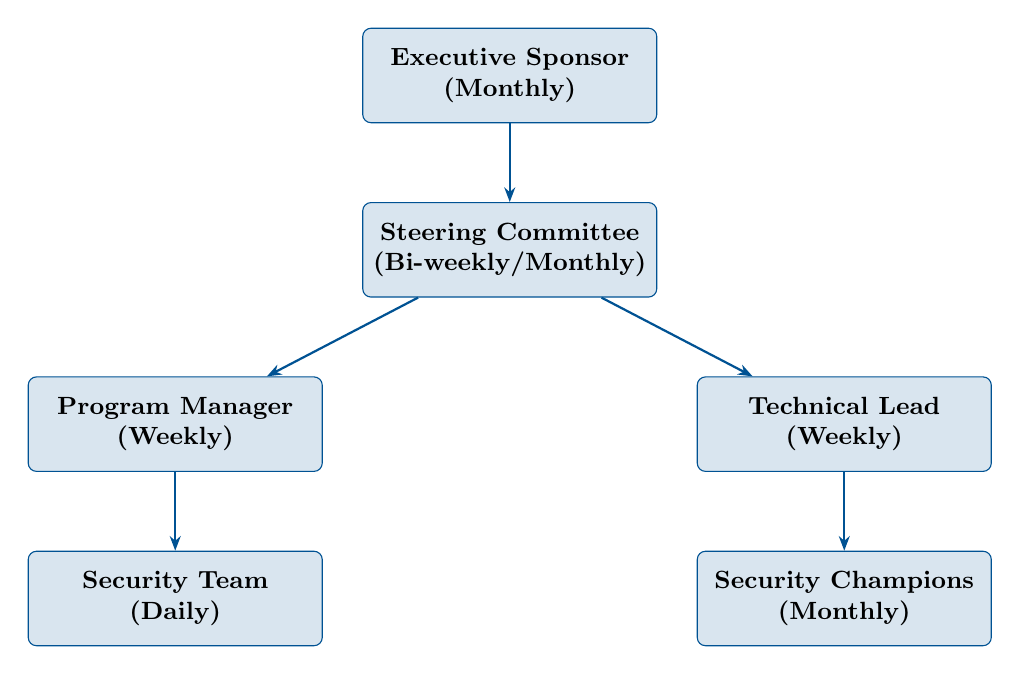
\begin{tikzpicture}[
    node distance=1cm,
    gov/.style={rectangle, draw=primaryblue, fill=primaryblue!15, rounded corners=3pt, text width=3.5cm, minimum height=1.2cm, align=center, font=\small\bfseries},
    arrow/.style={-{Stealth[scale=0.8]}, thick, primaryblue}
]
    \node[gov] (exec) {Executive Sponsor\\(Monthly)};
    \node[gov, below=of exec] (steering) {Steering Committee\\(Bi-weekly/Monthly)};
    \node[gov, below left=1cm and 0.5cm of steering] (program) {Program Manager\\(Weekly)};
    \node[gov, below right=1cm and 0.5cm of steering] (tech) {Technical Lead\\(Weekly)};
    \node[gov, below=1cm of program] (team) {Security Team\\(Daily)};
    \node[gov, below=1cm of tech] (champions) {Security Champions\\(Monthly)};
    
    \draw[arrow] (exec) -- (steering);
    \draw[arrow] (steering) -- (program);
    \draw[arrow] (steering) -- (tech);
    \draw[arrow] (program) -- (team);
    \draw[arrow] (tech) -- (champions);
\end{tikzpicture}
\caption{Roadmap Governance Structure}
\label{fig:governance-structure}
\end{figure}

\subsection{Reporting Cadence}

\begin{table}[H]
\centering
\renewcommand{\arraystretch}{1.3}
\begin{tabularx}{\textwidth}{>{\bfseries}p{3cm} p{2.5cm} X}
\toprule
\textbf{Report} & \textbf{Frequency} & \textbf{Content} \\
\midrule
Executive Dashboard & Monthly & High-level metrics; milestone status; key risks; budget status; strategic decisions needed \\
Steering Report & Bi-weekly & Detailed progress; issue resolution; upcoming activities; resource needs; risk updates \\
Program Status & Weekly & Task completion; blocker resolution; team activities; near-term plan \\
Metrics Report & Monthly & Full metrics dashboard; trend analysis; SLA compliance; coverage status \\
Phase Gate Review & Per phase & Phase completion assessment; success criteria validation; next phase readiness \\
Annual Assessment & Annually & Maturity assessment; program health; strategic review; roadmap update \\
\bottomrule
\end{tabularx}
\caption{Roadmap Reporting Cadence}
\label{tab:reporting-cadence}
\end{table}

\subsection{Phase Gate Reviews}

Conduct formal phase gate reviews before advancing to subsequent phases:

\begin{policybox}[Phase Gate Review Process]
\textbf{Review Preparation:}
\begin{itemize}[leftmargin=1.5em, itemsep=0.1em]
    \item Compile evidence for all success criteria
    \item Document any incomplete items with remediation plans
    \item Prepare updated risk assessment
    \item Finalize next phase plan and resource requirements
\end{itemize}

\textbf{Review Participants:}
\begin{itemize}[leftmargin=1.5em, itemsep=0.1em]
    \item Executive Sponsor
    \item Steering Committee members
    \item Program Manager
    \item Technical Lead
    \item Key stakeholder representatives
\end{itemize}

\textbf{Gate Decisions:}
\begin{itemize}[leftmargin=1.5em, itemsep=0.1em]
    \item \textbf{Proceed:} All success criteria met; proceed to next phase
    \item \textbf{Proceed with Conditions:} Minor gaps acceptable; proceed with remediation plan
    \item \textbf{Extend:} Significant gaps require additional time in current phase
    \item \textbf{Reassess:} Fundamental issues require roadmap revision
\end{itemize}
\end{policybox}

\subsection{Change Control}

\begin{table}[H]
\centering
\renewcommand{\arraystretch}{1.3}
\begin{tabularx}{\textwidth}{>{\bfseries}p{2.5cm} X p{3cm}}
\toprule
\textbf{Change Type} & \textbf{Examples} & \textbf{Approval Authority} \\
\midrule
Minor & Task reprioritization; minor timeline adjustment ($<$2 weeks); tool configuration changes & Program Manager \\
Moderate & Phase timeline extension (2-4 weeks); scope adjustment within phase; budget reallocation $<$10\% & Steering Committee \\
Major & Phase addition/removal; significant scope change; budget impact $>$10\%; strategic approach change & Executive Sponsor \\
\bottomrule
\end{tabularx}
\caption{Change Control Authority Matrix}
\label{tab:change-control}
\end{table}

% ============================================================================
% CONCLUSION
% ============================================================================
\section{Conclusion}

This Application Security Program Roadmap provides the comprehensive guidance necessary to systematically build and mature application security capabilities across the enterprise. The phased approach enables organizations to demonstrate value early while building toward comprehensive security coverage and operational excellence.

\begin{summarybox}
\textbf{Key Takeaways:}

\textbf{1. Phased Approach:} The five-phase structure provides a realistic path from initial capabilities to sustained excellence, with clear milestones and success criteria at each stage.

\textbf{2. Technology Agnostic:} The roadmap applies across any technology environment, enabling organizations to adapt activities to their specific technology landscape.

\textbf{3. Risk-Based Prioritization:} Focus resources on highest-risk applications first, expanding coverage systematically based on risk classification.

\textbf{4. Developer Integration:} Success depends on integrating security into developer workflows rather than imposing external gates that create friction.

\textbf{5. Measurable Progress:} Clear metrics and success criteria enable demonstration of value and identification of improvement opportunities.

\textbf{6. Sustained Investment:} Building mature security capabilities requires sustained commitment over multiple years, not a one-time project.

\textbf{7. Continuous Evolution:} The journey toward security excellence never truly ends; Phase 5 establishes the practices for ongoing improvement and adaptation.
\end{summarybox}

\vspace{1cm}

\begin{center}
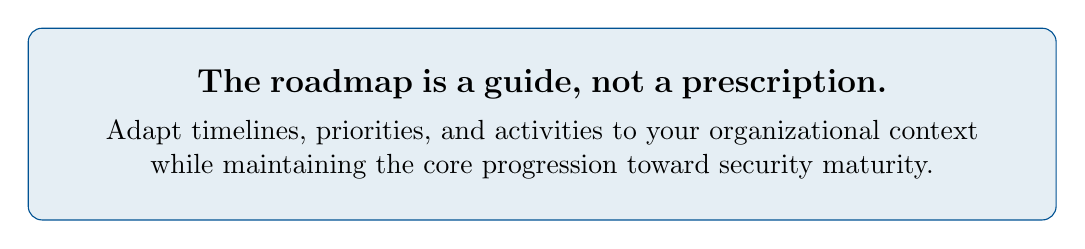
\begin{tikzpicture}
    \node[draw=primaryblue, fill=primaryblue!10, rounded corners=5pt, 
          text width=12cm, align=center, inner sep=15pt] {
        \textbf{\large The roadmap is a guide, not a prescription.}\\[0.5em]
        {\normalsize Adapt timelines, priorities, and activities to your organizational context\\while maintaining the core progression toward security maturity.}
    };
\end{tikzpicture}
\end{center}

% ============================================================================
% APPENDICES
% ============================================================================
\newpage
\appendix

\clearpage
\section{Appendix A: Phase Readiness Checklist}

Use this checklist to assess readiness to advance from each phase:

\begin{longtable}{>{\bfseries\raggedright\arraybackslash}p{3cm} p{9cm} c}
\toprule
\textbf{Phase} & \textbf{Readiness Criterion} & \textbf{Status} \\
\midrule
\endfirsthead
\toprule
\textbf{Phase} & \textbf{Readiness Criterion} & \textbf{Status} \\
\midrule
\endhead
\bottomrule
\endfoot
Phase 1 Complete & Executive sponsor actively engaged & $\square$ \\
 & All core policies approved and published & $\square$ \\
 & Vulnerability tracking system operational & $\square$ \\
 & Tier 1 applications under SAST/SCA testing & $\square$ \\
 & Security Champion in each major team & $\square$ \\
 & Baseline metrics established and reported & $\square$ \\
 & Phase 2 plan approved with resources & $\square$ \\
\midrule
Phase 2 Complete & Tier 1-2 applications under full testing & $\square$ \\
 & CI/CD integration complete for Tier 1-2 & $\square$ \\
 & Security gates enforced for Tier 1 & $\square$ \\
 & 100\% developer training completion & $\square$ \\
 & Threat modeling operational & $\square$ \\
 & SLA compliance $\geq$85\% & $\square$ \\
 & Phase 3 plan approved with resources & $\square$ \\
\midrule
Phase 3 Complete & Full portfolio coverage achieved & $\square$ \\
 & IAST deployed for Tier 1 & $\square$ \\
 & Security architecture process mature & $\square$ \\
 & SBOM generation automated & $\square$ \\
 & Compliance evidence automated & $\square$ \\
 & Level 3 maturity confirmed & $\square$ \\
 & Phase 4 plan approved with resources & $\square$ \\
\midrule
Phase 4 Complete & Developer satisfaction $\geq$4.0/5.0 & $\square$ \\
 & False positive rate $<$15\% & $\square$ \\
 & Auto-remediation operational & $\square$ \\
 & RASP deployed for Tier 1 & $\square$ \\
 & Security platform operational & $\square$ \\
 & SLA compliance $\geq$95\% & $\square$ \\
 & Level 4 maturity confirmed & $\square$ \\
\end{longtable}

\clearpage
\section{Appendix B: Tool Evaluation Criteria}

\begin{longtable}{>{\bfseries\raggedright\arraybackslash}p{3.5cm} p{9.5cm}}
\toprule
\textbf{Criterion} & \textbf{Evaluation Considerations} \\
\midrule
\endfirsthead
\toprule
\textbf{Criterion} & \textbf{Evaluation Considerations} \\
\midrule
\endhead
\bottomrule
\endfoot
Language Support & Coverage of languages in portfolio; quality of analysis per language; support for modern language features \\
Framework Support & Recognition of framework-specific patterns; understanding of framework security controls \\
Integration & CI/CD pipeline integration; IDE plugins; API availability; webhook support; SSO capability \\
Accuracy & False positive rate; false negative rate; contextual analysis capability \\
Performance & Scan speed; incremental scanning; resource consumption; scalability \\
Usability & Developer interface quality; finding clarity; remediation guidance; learning curve \\
Reporting & Dashboard capabilities; export options; trend analysis; customization \\
Administration & Rule customization; policy management; multi-tenant support; RBAC \\
Vendor Viability & Company stability; product roadmap; customer base; support quality \\
Total Cost & License costs; implementation effort; ongoing maintenance; training needs \\
\end{longtable}

\clearpage
\section{Appendix C: Key Metrics Reference}

\begin{longtable}{>{\bfseries\raggedright\arraybackslash}p{4cm} p{5cm} p{4cm}}
\toprule
\textbf{Metric} & \textbf{Definition} & \textbf{Target Trajectory} \\
\midrule
\endfirsthead
\toprule
\textbf{Metric} & \textbf{Definition} & \textbf{Target Trajectory} \\
\midrule
\endhead
\bottomrule
\endfoot
Vulnerability Density & Findings per 1000 lines of code & Decreasing \\
Mean Time to Remediate & Average days from discovery to resolution & Decreasing \\
SLA Compliance & Percentage of findings fixed within SLA & Increasing to $>$95\% \\
Open Vulnerability Count & Total open findings by severity & Critical/High: Decreasing \\
Security Debt Ratio & Open findings / Total findings discovered & Decreasing \\
Testing Coverage & Applications under active testing / Total applications & Increasing to 100\% \\
CI/CD Integration & Apps with pipeline security / Total apps & Increasing to 100\% \\
Training Completion & Developers trained / Total developers & Increasing to 100\% \\
False Positive Rate & Confirmed FP / Total findings & Decreasing to $<$15\% \\
Developer Satisfaction & Survey score (1-5 scale) & Increasing to $>$4.0 \\
Exception Rate & Active exceptions / Total vulnerabilities & Low and stable \\
Recurrence Rate & Reintroduced findings / Total fixed & Decreasing \\
\end{longtable}

\clearpage
\section{Appendix D: Communication Templates}

\subsection*{D.1 Executive Sponsor Communication}

\begin{policybox}[Monthly Executive Update Template]
\textbf{Application Security Program --- Monthly Update}

\textbf{Period:} [Month/Year]

\textbf{Overall Status:} [Green/Yellow/Red]

\textbf{Key Accomplishments:}
\begin{itemize}[leftmargin=1.5em, itemsep=0.1em]
    \item Accomplishment 1
    \item Accomplishment 2
    \item Accomplishment 3
\end{itemize}

\textbf{Key Metrics:}
\begin{itemize}[leftmargin=1.5em, itemsep=0.1em]
    \item Critical/High Vulnerabilities: [Count] ([Trend])
    \item SLA Compliance: [Percentage]
    \item Coverage: [Percentage] of portfolio
\end{itemize}

\textbf{Risks/Issues Requiring Attention:}
\begin{itemize}[leftmargin=1.5em, itemsep=0.1em]
    \item Issue 1 --- requested action
    \item Issue 2 --- requested action
\end{itemize}

\textbf{Next Month Focus:}
\begin{itemize}[leftmargin=1.5em, itemsep=0.1em]
    \item Priority 1
    \item Priority 2
\end{itemize}
\end{policybox}

\subsection*{D.2 Development Team Communication}

\begin{examplebox}[New Tool Rollout Announcement Template]
\textbf{Subject:} Application Security Tool Rollout --- [Tool Name]

\textbf{What's Happening:}
We are deploying [Tool Name] to help identify and fix security vulnerabilities earlier in development.

\textbf{When:}
[Rollout dates and phases]

\textbf{What You Need to Do:}
\begin{itemize}[leftmargin=1.5em, itemsep=0.1em]
    \item Action 1
    \item Action 2
\end{itemize}

\textbf{Training and Support:}
\begin{itemize}[leftmargin=1.5em, itemsep=0.1em]
    \item Training sessions: [dates/links]
    \item Documentation: [link]
    \item Support: [contact/channel]
\end{itemize}

\textbf{Questions?}
Contact your Security Champion or reach out to [security team contact].
\end{examplebox}

\clearpage
\section{Appendix E: Glossary of Terms}

\begin{longtable}{>{\bfseries}p{3.5cm} p{9.5cm}}
\toprule
\textbf{Term} & \textbf{Definition} \\
\midrule
\endfirsthead
\toprule
\textbf{Term} & \textbf{Definition} \\
\midrule
\endhead
\bottomrule
\endfoot
BSIMM & Building Security In Maturity Model --- framework for measuring software security initiatives \\
CI/CD & Continuous Integration / Continuous Deployment --- automated software delivery practices \\
CVE & Common Vulnerabilities and Exposures --- standardized vulnerability identifiers \\
CVSS & Common Vulnerability Scoring System --- standard for rating vulnerability severity \\
DAST & Dynamic Application Security Testing --- testing running applications for vulnerabilities \\
IAST & Interactive Application Security Testing --- runtime analysis combining static and dynamic techniques \\
OWASP & Open Web Application Security Project --- community producing security guidance and tools \\
RASP & Runtime Application Self-Protection --- security technology embedded in applications \\
SAMM & Software Assurance Maturity Model --- OWASP framework for software security practices \\
SAST & Static Application Security Testing --- analysis of source code for vulnerabilities \\
SBOM & Software Bill of Materials --- inventory of software components \\
SCA & Software Composition Analysis --- analysis of third-party and open-source components \\
SDLC & Software Development Life Cycle --- phases of software development \\
SLA & Service Level Agreement --- agreed remediation timeframes \\
SSDLC & Secure Software Development Life Cycle --- SDLC with integrated security activities \\
STRIDE & Threat modeling methodology: Spoofing, Tampering, Repudiation, Information Disclosure, Denial of Service, Elevation of Privilege \\
\end{longtable}

\end{document}
